% !TEX program = xelatex
% 컴파일: xelatex main.tex; bibtex main; xelatex main.tex; xelatex main.tex
% (Overleaf 사용 시 Compiler를 XeLaTeX 로 설정)
%
% 국내 학회 제출용 2단 축약본이다. 실험 절차와 부수 분석을 모두 담은 전체판은
% main_full.tex 에 있다.
\documentclass[10pt,twocolumn]{article}

\usepackage{kotex}          % 한국어
\usepackage[a4paper,top=20mm,bottom=22mm,left=19mm,right=19mm,columnsep=6mm]{geometry}
\usepackage{graphicx}
\usepackage{booktabs}
\usepackage{amsmath,amssymb}
\usepackage{array}
\usepackage{caption}
\usepackage{stfloats}       % 2단 조판에서 table* 를 페이지 하단에도 배치
\usepackage[hidelinks]{hyperref}
\usepackage{cite}

% 한글 이탤릭 폰트가 없어 \emph 의 기울임이 렌더링되지 않는다(로그의 UnBatang italic 미정의).
% 국내 학술지 관행에 맞추어 강조를 굵게로 바꾼다.
\renewcommand{\emph}[1]{\textbf{#1}}

\graphicspath{{figs/}}
\captionsetup{font=small,labelfont=bf,skip=4pt}
\renewcommand{\figurename}{그림}
\renewcommand{\tablename}{표}
\renewcommand{\refname}{참고문헌}

% 2단 좁은 행에서 한글 줄바꿈이 빡빡해지므로 여유를 준다.
\tolerance=2500
\emergencystretch=3em
\widowpenalty=10000
\clubpenalty=10000
\displaywidowpenalty=10000

% float 여백과 배치 규칙
\setlength{\textfloatsep}{8pt plus 2pt minus 2pt}
\setlength{\floatsep}{8pt plus 2pt minus 2pt}
\setlength{\intextsep}{8pt plus 2pt minus 2pt}
\setlength{\dblfloatsep}{8pt plus 2pt minus 2pt}
\setlength{\dbltextfloatsep}{10pt plus 2pt minus 2pt}
\renewcommand{\topfraction}{0.92}
\renewcommand{\bottomfraction}{0.8}
\renewcommand{\textfraction}{0.07}
\renewcommand{\floatpagefraction}{0.75}
\renewcommand{\dbltopfraction}{0.92}
\renewcommand{\dblfloatpagefraction}{0.7}
\setcounter{topnumber}{3}
\setcounter{bottomnumber}{2}
\setcounter{totalnumber}{5}
\setcounter{dbltopnumber}{3}

\title{STT 없이 음향 특징만으로 개인정보(PII) 형식 숫자열을 탐지하는 경량 CNN의 타당성 연구}
\author{김현찬 \quad 박승진 \quad 강진구}
\date{}

\begin{document}

% 주의: 아래 \twocolumn[...] 의 옵션 인자 안에서 중괄호 밖의 ']' 는 인자를 조기 종료시킨다.
% 수학식의 구간 표기처럼 ']' 를 써야 하면 {$[a, b]$} 처럼 중괄호로 감쌀 것.
\twocolumn[%
\begin{center}
{\LARGE\bfseries STT 없이 음향 특징만으로 개인정보(PII) 형식\\[2pt]
숫자열을 탐지하는 경량 CNN의 타당성 연구\par}
\vspace{4mm}
{\large 김현찬 \quad 박승진 \quad 강진구\par}
\vspace{1.5mm}
{\normalsize 숭실대학교 미디어학과\par}
\vspace{1mm}
{\small 2026년 8월\par}
\end{center}
\vspace{3mm}
\begin{center}
\begin{minipage}{0.9\textwidth}
\small
\noindent\textbf{요\ \ 약}\quad
음성에서 개인정보(Personally Identifiable Information, PII)를 찾는 표준 방식은
자동음성인식(Automatic Speech Recognition, ASR)으로 전사(Speech-to-Text, 이하 STT)한 뒤
자연어처리(Natural Language Processing, NLP)로 민감 정보를 탐지하는 캐스케이드이지만, 전사 비용과 지연, 전사 텍스트라는 새로운 유출 표면, 전사 오류의
후단 전파라는 세 비용을 치른다. 본 연구는 전사를 건너뛰고 멜 스펙트로그램에서 경량
합성곱신경망(Convolutional Neural Network, CNN)이 ``PII 형식 숫자열''의 포함 여부를 직접
판별하는 접근의 타당성을 통제 실험으로 검증한다. 지름길 단서를 차단한 한국어 합성
데이터셋에서 60{,}706 파라미터 CNN은 전화번호 단일 유형 통제 평가셋에서
$\text{F1}=0.955\pm0.010$을 얻어 음향 통계 로지스틱 회귀($0.761$)와 학습 가중치가 없는
온셋 연쇄 기준선($0.768$)을 능가하였고, PII 유형 넷·화자 14명 조건에서
$\text{F1}=0.859\pm0.011$, 재현율 $0.945\pm0.019$였다. 본 연구의 중심 결과는 성능 수치가
아니라 모델의 결정 함수를 특정한 것이다. 비PII 숫자열 카테고리를 하나씩 학습에서 제외하고
오탐률을 재면 12자리를 4-4-4로 끊어 읽는 제품 일련번호가 $0.947\pm0.041$로 최고인 반면
10자리를 끊지 않고 이어 읽는 주문번호는 $0.622\pm0.096$에 그치며, PII 의미가 없는 통제 자극
1{,}280개에서도 판정 비율은 자릿수에 대한 시그모이드(반포화점 $11.3$자리)이고 총 자릿수를
맞춘 채 그룹 구조만 바꾸어도 곡선이 겹친다($11.8$자리). 즉 모델이 재는 것은 그룹 형식이
아니라 자릿수 낭독의 분량이며, 관측된 정밀도 상한은 그 결정 축 위에서의 상한이다. 이 축이 전역
평균 풀링이 순서를 지운 결과인지도 검정하였다. 몸통을 고정한 채 헤드를 어텐션 풀링과 양방향
GRU로 바꾸고 시간 해상도를 네 배로 올려도 그룹 구조는 여전히 결정에 관여하지 않으며, 학습
분할에 자릿수 총량이 같고 그룹 구조만 다른 쌍이 직접 감독으로 들어 있는데도 그렇다. 다만 같은
축 위의 근사는 정밀해져 F1이 $0.859$에서 $0.932$로 오르므로, 보고한 수치는 접근법이 아니라
헤드의 한계이다. 일반화는
14화자 leave-one-speaker-out에서 $\text{F1}=0.871\pm0.085$, 학습에서 완전히 제외한 PII
유형에서 재현율 $0.89$--$0.92$로 성립하였다. Whisper 기반 STT+NLP와 동일 인스턴스에서
비교하면 16자리 카드번호 재현율이 네 디코딩 설정 모두에서 $0.802$--$0.864$인 반면 CNN은
$1.000$이고 정밀도는 반대로 $1.000$ 대 $0.787$이어서 두 경로의 실패 지점이 상보적이다. 클립 단위 판정을 실제로 결합하면 결합
방식이 결과를 가른다. 음향 경로를 앞단 필터로 두는 캐스케이드는 관례적 임계값 $0.5$에서 재현율이
STT 단독보다 낮지만(놓친 PII $23.3$건 대 $13.0$건) $\tau=0.1$에서는 손실 없이 STT 호출을 줄이며(가정한 콜센터형 트래픽에서 $39.9\%$, 모든 발화가
숫자를 포함하는 평가셋 자체에서는 $8.5\%$), 두 판정의 합집합은 놓친 PII를 $0.0$건으로 없앤다. 이를 근거로 음향 경로를
비용 프리필터와 재현율 안전망 양쪽으로 쓰는 결합과 그 손익분기 모형을 제시한다. 결과는 합성 음성에 한정되며, 8\,kHz 협대역과 G.711 코덱은 F1을 $0.859$에서
$0.831$로 낮추는 데 그치고 전화 통과대역으로 제한한 잡음에서는 SNR 20\,dB까지 재현율
$0.931$이 유지된다. 다만 같은 조건에서 STT+NLP가 $0.932$--$0.962$를 유지하므로 잡음 구간에서
프리필터가 더 많이 잃는다는 사실은 남는다. 또한 보고한 $\pm$는 학습 시드 분산일 뿐이며, 지배적 불확실성 축인 템플릿
구성을 부트스트랩으로 재면 F1의 95\% 구간이 {$[0.519, 0.960]$}으로 한 자릿수 넓다(재표집 단위가
여섯 그룹뿐이라 불확실성의 하한으로 읽어야 한다).

\vspace{2mm}
\noindent\textbf{핵심어:}\ 음성 개인정보 탐지, STT-free 음성 이해, 멜 스펙트로그램,
경량 합성곱신경망, 지름길 학습, 프리필터

\vspace{3mm}
\noindent\textbf{Abstract}\quad
The standard pipeline for detecting personally identifiable information (PII) in speech
transcribes every utterance with ASR and then applies NLP to the transcript. This cascade
pays three costs: transcription latency and price, a new leakage surface in the transcript
itself, and propagation of recognition errors. We test the feasibility of skipping
transcription altogether: a 60{,}706-parameter CNN decides directly from a log-mel
spectrogram whether an utterance contains a PII-formatted digit string. On a controlled
Korean synthetic corpus built to block shortcut cues, the model reaches $\text{F1}=0.955$ on
a single-type (phone number) test set and $0.859$ with four PII types and 14 speakers. Our
central result is not the score but an identification of what the model measures. A
held-out-category false-positive analysis and 1{,}280 semantically meaningless controlled
digit stimuli show that the decision variable is the \textit{amount} of isochronous
monosyllabic digit reading (logistic half-saturation at $11.3$ digits), not the grouping
structure of the format: matching total digit count while regrouping into
four-digit blocks leaves the curve unchanged ($11.8$ digits). The observed precision ceiling
is therefore a ceiling on that decision axis rather than a limit of the task. Against a
Whisper-based STT+NLP path on identical instances, the two approaches fail in complementary
places (16-digit card recall $1.000$ vs. $0.802$--$0.864$; precision $0.787$ vs. $1.000$),
motivating a two-stage prefilter-then-verify pipeline and its break-even model. All results are
obtained on TTS-synthesised speech; narrowband and G.711 degradation cost little (F1 $0.859$ to
$0.831$), but validation on real recordings remains open.

\vspace{2mm}
\noindent\textbf{Keywords:}\ speech PII detection, STT-free spoken language understanding,
mel-spectrogram, lightweight CNN, shortcut learning, prefilter
\end{minipage}
\end{center}
\vspace{4mm}
]

\section{서론}\label{sec:intro}

콜센터 상담, 회의 녹취, 음성 메모 등 음성 데이터에는 전화번호, 주민등록번호, 계좌번호,
카드번호와 같은 개인정보(Personally Identifiable Information, PII)가 빈번하게 포함된다.
현재 표준적인 접근은 음성을 자동음성인식(Automatic Speech Recognition, ASR)으로 전사한 뒤
전사 텍스트에 개체명 인식이나 정규식 패턴 매칭을 적용해 민감 구간을 찾고 그 구간에
대응하는 오디오를 마스킹하는 캐스케이드 파이프라인이며~\cite{cohn2019audiodeid}, 주요 상용
서비스와 실시간 상담 시스템이 모두 이 구조를 채택하고 있다~\cite{azurepii,gouvea2023trustera}.
이하에서는 전사 단계를 관례에 따라 STT(Speech-to-Text)로도 부르며 ASR과 같은 뜻으로
사용한다.

이 구조는 세 지점에서 비용을 치른다. 첫째, PII 포함 여부와 무관하게 모든 발화를 전사해야
하므로 대량 녹취를 다룰수록 STT 호출 비용이 선형으로 증가한다. 본 연구에서 측정한
Whisper-large-v3~\cite{radford2023whisper}의 전사 지연은 클립당 $0.54$--$0.67$초인 반면
뒤에서 제안할 경량 합성곱신경망(Convolutional Neural Network, CNN)의 추론 지연은 5초 윈도당
$0.344$\,ms이다. 다만 이 배수 자체가 운용 이득은 아니며, 실제 절감은 프리필터가 얼마나 많은
발화를 걸러 내는지에 달려 있으므로 \ref{sec:discuss:cost}절에서 트래픽 구성을 넣은 비용
모형으로 따로 계산한다. 둘째, 탐지 과정 자체가 민감 텍스트를 중간 산출물로 남긴다. 전사
텍스트는 PII를 평문으로 담아 로그, 캐시, 저장소 전반에 새로운 유출 표면을 만들며, 공개된
상담 전사 데이터셋들이 배포 전에 별도의 비식별화 공정을 거쳐야 하는 이유도 여기에
있다~\cite{dao2025callcenter}. 셋째, 전사 오류가 그대로 후단으로 전파된다. 본 연구의 비교
실험에서도 일반 발화의 단어오류율(Word Error Rate, WER) 중앙값이 0인 합성음 조건에서조차
숫자열 구간에서는 자릿수의 병합과 분절이 발생하여 16자리 카드번호에 대한 STT+NLP 재현율이 기본 디코딩 설정에서 $0.864$에 그쳤다. 전사 품질 전반이 좋더라도 오류가 하필 숫자열 구간에 집중된다는 뜻이다.

본 연구의 출발점은 다음 관찰이다. PII로 취급되는 숫자열은 낭독될 때 개별 숫자가 일정한
리듬으로 연속되고 자릿수 그룹 사이에 짧은 휴지가 놓인다. 이 규칙성은 소리를 멜
스펙트로그램\footnote{소리를 가로축 시간, 세로축 주파수의 2차원 이미지로 바꾼 표현이다. 사람
귀가 주파수를 인지하는 방식(멜 척도)에 맞추어 세로축을 눌러 놓은 것으로, 음성 처리에서 가장
널리 쓰이는 입력 형태이다. Whisper 같은 음성인식 모델도 같은 형태의 입력을 받는다.}로 바꾸어
보면 눈으로도 구분되는 무늬로 나타난다(그림~\ref{fig:melspec}). 이 가설이 성립한다면 ``어떤 숫자가 발화되었는가''라는 어휘
정보를 복원하지 않고도 ``숫자열이 PII의 형식을 띠는가''라는 비어휘적 패턴을 음향 표현만으로
판별할 수 있고, 전사 없이 동작하는 저비용 선별기를 캐스케이드 앞단에 배치하여 위의 세
비용을 동시에 완화할 수 있다. 이를 검증하기 위해 다섯 가지 연구 질문(Research Question,
RQ)에 답한다. STT 없이 음향 특징만으로 탐지가 가능한가(RQ1). 그 성능이 무엇에서 오는가. 즉 발화 길이나 ``숫자가 들리는가'' 같은
지름길 단서\footnote{모델이 과제의 본질 대신 데이터에 우연히 딸려 온 쉬운 단서로 답을 맞히는
현상을 shortcut learning이라 한다~\cite{geirhos2020shortcut}. 예컨대 PII가 든 문장만 유독
길게 만들어 두면 모델은 형식이 아니라 길이만 보고도 높은 점수를 낸다.}를 배제한 뒤 남는
신호가 정말 ``PII의 형식''인지, 아니면 더 단순한 무엇인지를 \emph{측정}할 수 있는가(RQ2). 학습에 없던 화자와 학습에서 제외한 PII 유형으로 일반화되는가(RQ3). 표준 경로인
STT+NLP와 비교했을 때 어떤 운용 위치가 합리적인가(RQ4). 이 과제에 적합한 모델 규모는
어디인가(RQ5).

본 연구의 기여는 다음 다섯 가지이다. (i) STT-free 음향 PII \emph{형식} 탐지 과제를
정식화하고, 지름길 단서를 차단한 통제 데이터셋과 템플릿 누수 없는 평가 프로토콜을
설계하였다. (ii) 길이 불변, ``숫자 존재''--``형식'' 분리, 캐리어 문장의 조건부 검정이라는
세 겹의 통제로 성능이 지름길 단서로 설명되지 않음을 보이고, 나아가 \emph{모델의 결정 함수를
직접 특정}하였다. 카테고리별 미학습 오탐률과 통제 자극 실험은 결정 변수가 그룹 구조가 아니라
등간격 단음절 연쇄의 분량임을 보이며, 이는 현재 모델이 도달한 정밀도 상한이 어느 축 위에
놓여 있는지를 정량화한다. (iii) 화자(LOSO)와 PII 유형(held-out) 두 축의 일반화를 검증하였다.
(iv) STT+NLP 표준 경로와 동일 조건, 네 가지 디코딩 설정에서 직접 비교하여 긴 숫자열에 대한
전사 취약성이 설정 미조정이 아님을 확인하고, 클립 단위 판정을 결합해 캐스케이드가 아니라 합집합이
이 상보성을 쓰는 결합임을 보이고 손익분기 모형을 제시하였다. (v) 모델별 학습률 스윕을 수행하여 60{,}706 파라미터 CNN이 각
모델에 가장 유리한 학습률에서도 27.8M ImageNet 백본을 능가함을 보이고, 협대역·코덱·잡음
열화를 실측하여 잡음을 전화 통과대역으로 제한해야 표적 도메인의 조건이 됨을 밝혔다.

\begin{figure*}[!t]
\centering
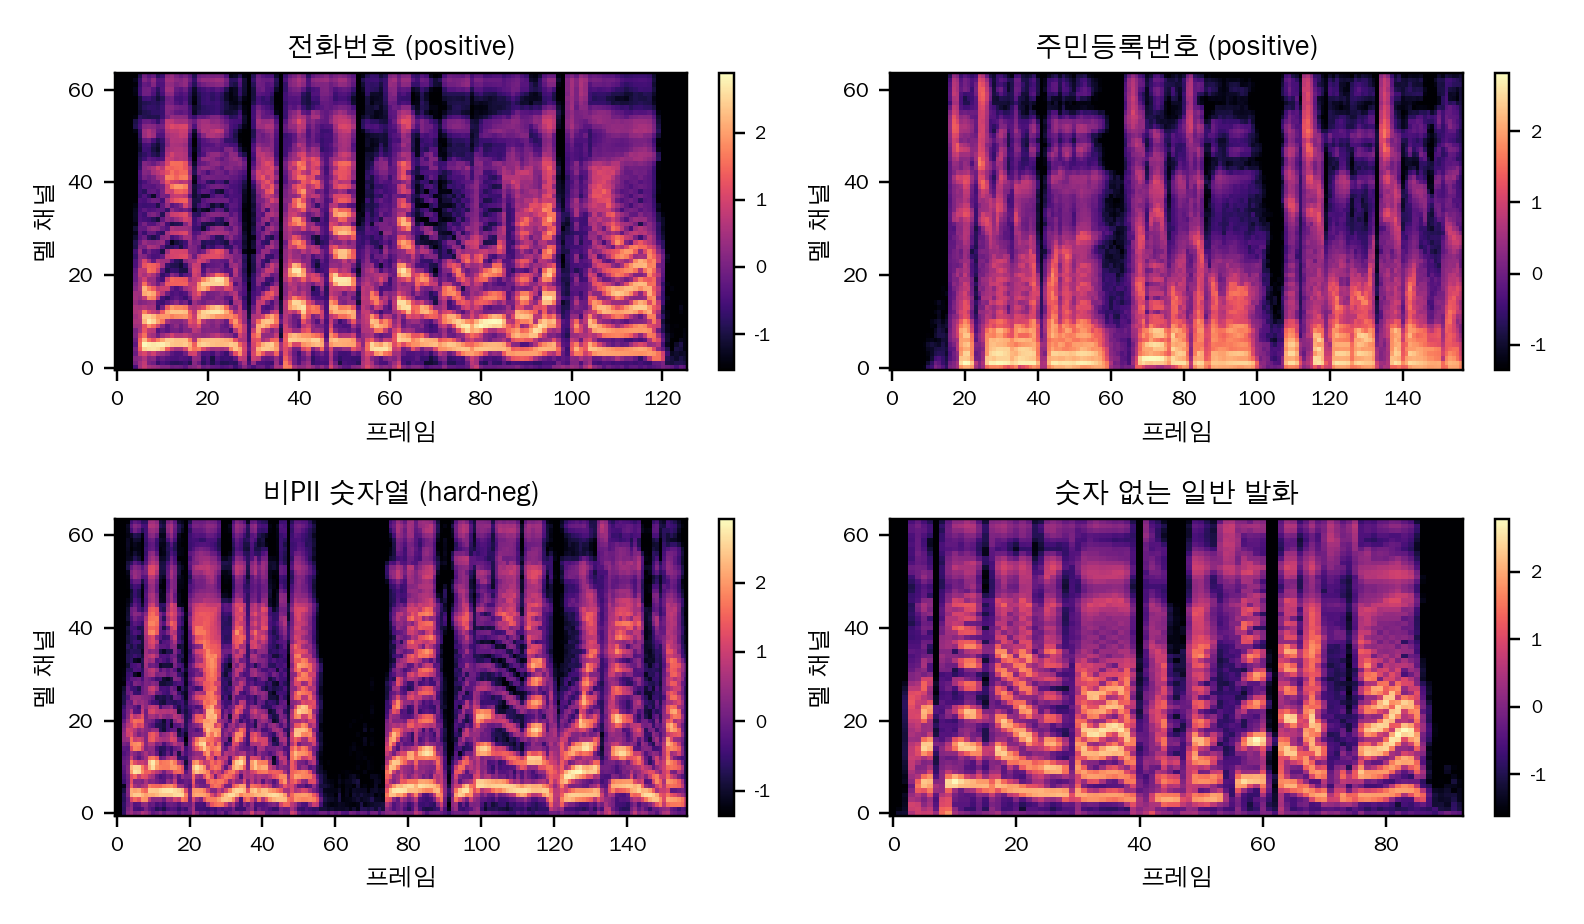
\includegraphics[width=\linewidth]{melspec_examples.png}
\caption{멜 스펙트로그램 예시. v2 데이터의 네 클립(전화번호 positive, 주민등록번호 positive,
hard-negative 숫자열, 숫자 없는 일반 발화)의 첫 5초 윈도를 모델 입력과 동일하게 변환한
것이다(멜 채널 64, 윈도별 표준화 후의 값). 자릿수로 낭독되는 PII 형식 숫자열은 규칙적인
시간-주파수 패턴(세로 줄무늬)으로 나타난다. 이 네 클립을 학습에서 제외한 뒤 실제로 추론했을 때
모델이 부여한 PII 확률은 각각 0.973, 0.989, 0.107, 0.030으로 네 건 모두 정답이었으므로, 그림의
텍스처 차이는 사후 해석이 아니라 모델의 판정과 일치한다.}
\label{fig:melspec}
\end{figure*}

\section{관련 연구}\label{sec:related}

\paragraph{캐스케이드 기반 음성 비식별화.}
음성에서 PII를 제거하는 문제는 Cohn 등~\cite{cohn2019audiodeid}이 오디오 비식별화라는 개체명
인식 과제로 정식화하였다. 이들은 ASR 전사, 개체명 인식, 오디오 구간 정렬의 세 단계
파이프라인과 그에 맞는 평가 지표를 제안했으며 이 구조가 이후 상용 시스템의 사실상 표준이
되었다~\cite{azurepii}. Trustera~\cite{gouvea2023trustera}는 이를 실시간 상담으로 확장하여
상담원이 카드번호를 듣지 않도록 하면서 대화의 자연스러움을 유지한다. 이러한 시스템이
공통적으로 안는 구조적 취약성은 텍스트 단계가 ASR 출력에 전적으로 의존한다는 데 있다. 구어
숫자는 발화 속도와 휴지에 따라 다르게 전사되고, 하나의 번호가 여러 토큰이나 여러 발화
구간으로 분절되며, 숫자 하나가 누락되어도 형식 매칭이 실패한다. 본 연구는 이 캐스케이드를
대체하려는 것이 아니라 그 앞단에 전사 없이 동작하는 경량 선별기를 두어 호출량과 유출 표면을
함께 줄이는 것을 목표로 한다.

\paragraph{ASR-free / 종단간 음성언어이해.}
방법론적으로 가장 가까운 계보는 음성에서 의미를 ASR 없이 직접 추론하는 종단간 음성언어이해
(Spoken Language Understanding, SLU)이다. Serdyuk 등~\cite{serdyuk2018towards}은 전사
텍스트를 거치지 않고 음향 특징에서 곧바로 의도를 예측하는 구조가 가능함을 보였고, Lugosch
등~\cite{lugosch2019pretrain}은 ASR 사전학습 인코더를 SLU로 전이하였으며, Palogiannidi
등~\cite{palogiannidi2020asrfree}은 사전학습 모델 없이 순환 구조와 증강만으로도 경쟁력 있는
결과를 얻었다. Tomashenko 등~\cite{tomashenko2019recent}은 음성에서 직접 개체명 인식과 슬롯
채우기를 수행하기 위한 화자 적응과 학습 기준 변형을 제안했고, 최근에는 자기지도 인코더에
연결주의 시간 분류(Connectionist Temporal Classification, CTC) 보조 손실을 결합하는 접근도
제안되었다~\cite{wang2023jointctc}. 전사 단계를 제거하면 ASR 오류가 후단으로 전파되지 않고
시스템이 단순해진다는 동기는 본 연구와 겹치나, 네 가지가 다르다. 첫째, 기존 SLU의 라벨은
의도나 슬롯처럼 \emph{어휘에 대응되는} 의미 범주인 반면 본 연구의 라벨은 ``PII 형식 숫자열의
존재''라는 비어휘적 상위 패턴이며, 어떤 숫자가 발화되었는지는 라벨과 무관하다. 둘째, 본
연구의 모델은 뒤따르는 정밀 파이프라인의 호출량을 줄이는 \emph{프리필터}이므로 균형 잡힌
정확도보다 고재현율과 초저지연이라는 비대칭적 운용점이 중요하다. 셋째, 평가의 초점이 벤치마크
점수가 아니라 높은 점수가 지름길 단서에서 오지 않았음을 보이는 통제에 있다. 넷째, 기존
종단간 SLU가 수천만에서 수억 파라미터의 사전학습 인코더를 쓰는 데 반해 본 연구는 60{,}706
파라미터 전용 CNN을 처음부터 학습한다. 또한 PII 형식 라벨과 통제된 hard-negative를 함께 갖춘
한국어 음성 데이터는 공개된 바 없어 기존 SLU 벤치마크를 재사용할 수 없다.

\paragraph{키워드 스포팅과 경량 음향 분류.}
멜 스펙트로그램과 소형 신경망으로 특정 어휘를 저전력에서 탐지하는 키워드 스포팅(Keyword
Spotting, KWS)은 본 연구가 사용하는 구현 기법을 공유한다. Sainath와
Parada~\cite{sainath2015cnnkws}는 CNN이 완전연결 신경망보다 훨씬 적은 파라미터로 더 낮은
오거부율을 달성함을 보였고, Tang과 Lin~\cite{tang2018resnetkws}, Berg
등~\cite{berg2021keyword}이 잔차 연결과 자기어텐션으로 이를 확장하였으며, 후속 연구는 대부분
고립 단어 코퍼스~\cite{warden2018speech}에서 평가된다. 대규모 오디오 분류에서는 AudioSet
사전학습 CNN~\cite{kong2020panns}이나 스펙트로그램 트랜스포머~\cite{gong2021ast}가 표준
표현으로 자리 잡았으나 파라미터가 수천만 개에 달해 상시 동작 프리필터의 예산에 맞지 않는다.
본 연구는 KWS와 기술적 구성에서도 구분된다. KWS는 고정 어휘의 각 항목에 대응하는 짧은 음향
앵커를 학습하지만 본 연구의 탐지 대상에는 그런 앵커가 없으며, 판별에 쓰이는 신호는 개별
숫자의 정체가 아니라 숫자 낭독 구간의 지속 길이와 리듬이라는 시퀀스 구조이다. 결정적으로 본
연구의 positive와 hard-negative는 \emph{동일한 숫자 어휘 집합}으로 이루어져 있어, 어떤 숫자
단어가 등장했는지만 판정하는 KWS식 어휘 집합 탐지로는 두 클래스를 분리할 수 없다. 그 때문에
어휘 단위 사후확률 설계 대신 윈도 최댓값 집계와 hard-negative 통제가 요구된다.

\paragraph{음성 콘텐츠 프라이버시.}
음성 프라이버시 연구는 화자 신원 은닉에서 출발하여 최근 발화 내용 자체의 보호로 확장되고
있다. Williams 등~\cite{williams2022content}은 음성이 단어와 의미뿐 아니라 문체, 병리적 특징,
감정까지 드러낸다는 점에서 콘텐츠 프라이버시가 별도의 과제임을 지적한다.
Preech~\cite{ahmed2020preech}는 전사 파이프라인 자체를 프라이버시 보존적으로 재구성하여
음성을 분절·치환한 뒤 외부 전사 서비스에 보내고 결과를 복원한다. 본 연구는 보호 지점이
다르다. Preech가 ``전사를 하되 안전하게 하는'' 접근이라면 본 연구는 ``대부분의 발화에 대해
전사 자체를 하지 않는'' 접근으로, 탐지 단계에서 이진 신호만 산출하여 민감 텍스트가 생성되는
사건 수를 줄인다. 두 접근은 배타적이지 않으며 프리필터를 통과한 소수의 발화에 프라이버시
보존 전사를 적용하는 결합도 가능하다. 요컨대 본 연구는 텍스트를 생성하지 않는다는 점에서
종단간 SLU 및 KWS와 같은 쪽에 서지만 라벨이 어휘가 아닌 \emph{형식}이라는 점에서 두 계보
모두와 갈라지며, 성능 수치보다 그 수치가 지름길 단서에서 오지 않았음을 보이는 통제에 지면을
배분한다는 점에서 벤치마크 경쟁형 연구와 목적이 다르다.

\section{과제 정식화 및 데이터셋}\label{sec:data}

\subsection{과제 정의}
과제를 말로 먼저 적으면 이렇다. 긴 녹음을 5초짜리 조각으로 잘라 각 조각이 PII 형식 숫자열을
담고 있는지 0에서 1 사이 점수로 매기고, 조각들의 점수 가운데 가장 높은 값을 그 녹음 전체의
점수로 삼는다. 가장 높은 값을 쓰는 이유는 녹음 어디에 숫자열이 있든 놓치지 않기 위해서이다.

형식적으로는 다음과 같다. 입력은 5초 음향 윈도의 로그 멜 스펙트로그램
$\mathbf{X}\in\mathbb{R}^{64\times157}$이며(멜 채널 64, hop 512 표본에서 유도되는 프레임 수
157), 모델은 윈도가 PII 형식 숫자열을 포함할 확률
$f(\mathbf{X})=\mathrm{softmax}(g(\mathbf{X}))_1\in[0,1]$을 출력한다. 여기서 $g$는
2차원 로짓을 내는 신경망이다. 클립 $c$에 대해 $W(c)$는 그 클립을 2.5초 간격의 sliding
window로 덮어 얻은 5초 윈도들의 집합이며(클립이 5초보다 짧으면 저진폭 노이즈로 패딩한 윈도
한 개), 클립 점수는 $s(c)=\max_{\mathbf{X}\in W(c)} f(\mathbf{X})$로 정의한다. 최종 판정은
임계값 $\tau$에 대해 $\hat{y}(c)=\mathbb{1}[s(c)\ge\tau]$이며, 별도로 밝히지 않는 한
$\tau=0.5$를 사용한다. 프리필터 관점에서 $\Pr[s(c)\ge\tau]$는 후단 STT로 넘어가는 클립의
비율, 즉 STT 호출률에 해당한다.

Positive는 전화번호, 주민등록번호, 계좌번호, 카드번호를 포함한 발화이고, negative는 PII가
아닌 숫자열을 포함한 hard-negative와 숫자열이 핵심 정보가 아닌 일반 발화
easy-negative로 구성한다.\footnote{hard-negative는 정답이 ``아니오''이면서도 모델이 헷갈리기
쉽게 만든 표본을 뜻한다. 여기서는 주문번호나 일련번호처럼 PII가 아니면서 숫자가 길게 들리는
발화가 이에 해당한다. easy-negative는 숫자가 아예 없어 쉽게 걸러지는 일반 발화이다. 두 종류를
나누어 세는 이유는, 전체 오탐률만 보면 easy-negative가 많을수록 성적이 좋아 보여 모델의 실제
어려움이 가려지기 때문이다.} 본 과제는 ``문맥상 실제로 민감한가''가 아니라 ``PII 형식 숫자열이 음향적으로
존재하는가''를 판별하는 것으로 한정한다. 따라서 ``이건 예시 번호입니다''처럼 문맥상 실제
PII가 아니더라도 형식이 들리면 positive로 라벨링한다. 문맥 판단은 \ref{sec:exp}장에서
비교하는 STT+NLP 단계의 역할이며, 본 모델은 그 앞단의 형식 선별기이다.

\subsection{데이터 생성과 지름길 단서 통제}\label{sec:data:gen}
PII가 포함된 실제 음성은 정의상 수집·공개가 불가능하므로 통제 가능한 합성 음성 데이터셋을
직접 구축하였다. 이하는 v2를 기준으로 서술한다.

\paragraph{문장과 값 생성.}
PII 유형별로 문장 템플릿을 두고(전화 5종, 주민 4종, 계좌 4종, 카드 3종) 각 발화마다 형식만
유효한 난수 값을 생성하여 삽입한다. 전화번호는 3-4-4(11자리), 주민등록번호는 6-7(13자리),
계좌번호는 3-3-6(11--12자리), 카드번호는 4-4-4-4(16자리) 형식이며 값은 난수이므로 실재하는
번호가 아니다. hard-negative는 날짜, 주문번호(9--11자리), 송장번호(4-4), 가격, 우편번호,
좌석번호, 제품 일련번호(4-4-4), 생일, 버스번호, 수 세기의 10개 카테고리 생성기로 만들며,
우연히 전화번호 형식이 만들어지면 정규식으로 검출해 재생성한다. easy-negative는 숫자를
포함하지 않는 12종의 일반 문장이다. v1은 전화번호 단일 유형만 다루며, 숫자열을 문장
앞·중간·끝에 배치한 일반 템플릿 10종과 문맥상 실제 PII가 아니지만 형식은 들리는 문맥 변형
템플릿 4종(전체의 20\%)으로 이루어진다.

\paragraph{읽기 방식 통제.}
한국어에서 숫자는 자릿수를 하나씩 읽는 방식(``공일공 일이삼사'')과 수량으로 읽는
방식(``삼만 오천 원'')의 두 가지로 낭독된다. 자연스럽게 합성하면 전화번호와 계좌번호는 자릿수
읽기로, 가격과 날짜는 수량 읽기로 낭독되어 두 클래스의 음소 구성과 운율이 체계적으로
달라지고, 모델은 ``PII 형식인가''가 아니라 ``자릿수 읽기인가''라는 훨씬 쉬운 지름길만으로
두 클래스를 분리할 수 있다. 이를 막기 위해 클래스를 가리지 않고 문장 안의 \emph{모든} 숫자를
자릿수 발음으로 강제 변환하였다. 예컨대 hard-negative의 ``오늘은 2026년 3월 25일입니다''는
``오늘은 이공이육년 삼월 이오일입니다''로, positive의 ``카드번호는
4921-3387-0155-2860입니다''는 ``카드번호는 사구이일 삼삼팔칠 공일오오 이팔육공입니다''로
합성된다. 그 결과 두 클래스는 사용하는 음소 목록과 낭독 스타일이 사실상 동일해지고, 남는
차이는 오직 숫자열의 형식뿐이다. 다만 hard-negative의 ``수 세기''(``하나 둘 셋 넷 다섯'')는
아라비아 숫자를 포함하지 않아 변환 대상이 아니며, 고유어 수사가 연속될 때에도 오탐이
발생하는지를 보기 위한 별도 조건으로 포함하였다.

\paragraph{hard-negative 설계.}
negative가 숫자를 포함하지 않는 일반 발화뿐이라면 ``숫자 소리가 들리는가''라는 단일 규칙만으로
높은 정확도가 나오므로, 숫자를 포함하되 PII가 아닌 발화를 negative의 상당 부분으로 투입하였다.
특히 v2에서는 주문번호를 9--11자리, 제품 일련번호를 4-4-4자리로 설계하여 각각 계좌·전화번호,
카드번호와 자릿수 길이 및 그룹 구조가 의도적으로 충돌하게 만들었다. 이들은 앞의 읽기 방식
통제에 따라 positive와 동일하게 자릿수로 낭독되므로 ``숫자 존재''는 두 클래스 사이에서 상수가
되며, 결과적으로 hard-negative에 대한 오탐률(False Positive Rate, FPR)이 모델이 숫자의 유무를
넘어 무엇을 재고 있는지를 직접 측정하는 지표가 된다. 형식적으로
$\frac{1}{|H|}\sum_{c\in H}\mathbb{1}[s(c)\ge\tau]$로 정의하며 $H$는 평가셋의 hard-negative
클립 집합이다. 분모가 negative 전체가 아니라는 점에서 통상의 FPR과 다르다.

\paragraph{길이 정렬과 캐리어 문장.}
hard-negative의 핵심 문장은 positive보다 짧아 그대로 두면 클립 길이가 클래스 단서가 된다.
이를 막기 위해 hard-negative에는 85\% 확률로 ``안내 말씀드립니다'' 같은 숫자 없는 안내 문구를
앞이나 뒤에 결합하였다. 실제로 v2 hard-negative의 길이 중앙값은 캐리어가 붙은 경우 4.72초,
붙지 않은 경우 3.04초로 캐리어가 positive의 4.56초에 길이를 맞추는 역할을 한다. positive에는
캐리어를 붙이지 않는 대신 숫자열이 문장 앞·중간·끝에 오도록 여러 템플릿을 사용하여 절대
위치가 단서가 되지 않게 하였다. 캐리어가 hard-negative 쪽에 치우쳐 나타나므로(v2 기준
hard-negative의 87.1\%, 나머지 0\%) ``캐리어가 들리면 negative''라는 지름길 가능성이 남는데,
이는 \ref{sec:exp}장에서 조건부 오탐률로 직접 검정하며 \emph{부호가 반대}로 기각된다. 5초보다
짧은 클립은 무음이 아니라 진폭 $10^{-3}$의 저진폭 노이즈로 패딩하여 무음 길이가 원 클립
길이를 노출하지 않게 하였고, 세 클래스를 모두 동일한 화자 풀, 동일한 TTS 모델, 동일한
후처리(16\,kHz 모노)로 생성하여 코덱 특성이나 화자 지문이 단서가 되지 않게 하였다.

\paragraph{음성 합성과 화자 은행.}
v1은 음성합성(Text-to-Speech, TTS) 도구인 edge-tts의 한국어 신경망 음성 3종으로,
v2는 Qwen3-TTS~\cite{hu2026qwen3tts} 기반의
14화자 음성 은행으로 합성한다. 화자 은행은 두 단계로 만들었다. 먼저 VoiceDesign 체크포인트에
``20대 여성, 높고 밝은 목소리, 빠른 말투'' 같은 한국어 지시문을 주어 화자마다 고정된 문장 한
개를 합성해 참조 음성으로 저장하고(성별 7:7, 연령 20--60대), 데이터셋의 1{,}800개 발화는 모두
Base 체크포인트의 음성 복제 기능으로 합성하였다. VoiceDesign을 발화마다 직접 호출하면 같은
지시문에도 음색 변동이 커서 화자 간/화자 내 임베딩 거리 비가 $0.61$에 그쳤으나, 참조 음성
1개를 고정해 복제하자 $2.29$로 개선되었다. 이 값은 데이터를 만든 Base 모델의 \emph{내부}
임베딩으로 잰 것이므로, 화자 임베딩 계열의 후속 모델인
ECAPA-TDNN~\cite{desplanques2020ecapa}(x-vector~\cite{snyder2018xvector}의 후속)으로 다시
확인하였다. 화자당 30개 클립에서 화자 내 평균 코사인 거리 $0.242$, 화자 간 중심 거리 평균
$0.506$으로 비율은 $2.09$로, 척도는 달라도 결론은 유지된다. 다만 가장 가까운 쌍의 거리가
$0.179$로 화자 내 평균보다 작아 14화자 중 두 명은 독립 검증 기준으로 충분히 분리되지 않는다.
v2에서는 화자를 발화 순서에 따라 균등 순환 배정하여 클래스와 화자가 상관되지 않게 하였고
(화자별 128--131개), 모든 출력은 16\,kHz 모노 PCM16으로 통일하였다. 생성 난수 시드는 42로
고정하였다(v1 hard-negative만 43).

\paragraph{윤리적 고려.}
사용된 모든 음성은 TTS 합성이며 실제 인물의 음성을 포함하지 않는다. 발화에 등장하는 번호는
형식만 맞춘 난수로 실재하는 개인의 정보가 아니므로 데이터 수집 단계에서 개인정보가 처리되지
않았다.

\subsection{데이터셋 구성과 분할}\label{sec:data:split}
표~\ref{tab:data}에 두 버전의 구성과 분할 결과를 정리하였다. v1은 전화번호 단일 유형에 대한
통제 실험용, v2는 PII 유형과 화자를 함께 확장한 일반화 실험용이다. 클립 길이는 v2 기준
positive 중앙값 4.56초, hard-negative 4.64초, easy-negative 3.28초로 클래스 간 큰 편차가 없다.
v1의 easy-negative는 일반 발화 코퍼스 331종을 재사용한 것인데, 그 가운데 283종이 ``육삼팔번
버스''처럼 자릿수로 낭독되는 짧은 숫자 표현을 포함한다. 따라서 ``숫자 존재'' 단서를 두 클래스
사이에서 상수로 만든다는 통제 취지는 v1에서 오히려 더 강하게 성립한다.

분할은 클립 단위가 아니라 \emph{문장 템플릿 단위}로 수행한다. 이유는 간단하다. 같은 템플릿에서
나온 클립들은 숫자 값만 다르고 문장 뼈대가 똑같다. 예컨대 ``제 전화번호는 \{v\}입니다''라는
템플릿에서 나온 200개 클립을 학습과 평가에 나눠 넣으면, 모델은 형식을 배우지 않고 그 문장
자체를 외운 뒤 평가에서 맞힐 수 있다. 점수는 올라가지만 새 문장에는 통하지 않는다. 따라서 각 템플릿 식별자를 하나의 그룹으로 묶어 통째로 한 분할에만
배정한다(template-disjoint). 목표 비율은 70/15/15이며 라벨별로 목표량을 따로 채워 클래스
균형을 유지하고(label-stratified), 배정 순서는 그룹의 평균 길이 오름차순으로 하여 세 분할이
길이 스펙트럼을 고르게 나눠 갖게 한다(length-stratified). test 분할은 학습, 하이퍼파라미터
선택, 조기 종료, 임계값 결정 어디에도 사용하지 않는다. 임계값은 목적에 따라 세 규칙으로
정하는데, 메인 성능표와 통제 평가는 튜닝 없이 $0.5$를 쓰고, LOSO의 튜닝 임계값은 각 폴드의
검증 분할에서 F1을 최대화하는 값을, 프리필터 운용표의 임계값은 검증 분할에서 목표
재현율을 달성하는 지점의 점수를 그대로 가져다 쓴다. 예컨대 재현율 0.95를 원하면, 검증 분할의
PII 클립 가운데 95\%가 그 값 이상이 되는 점수를 임계값으로 삼는다. 세 규칙 모두 test를 참조하지 않는다.

v2에서는 템플릿 그룹화가 평가 분할의 구성을 결정한다. easy-negative 450개는 모두 하나의 템플릿
식별자를 공유하여 한 덩어리로 학습 분할에 배정되었고, hard-negative는 템플릿 식별자가 생성
카테고리 이름이어서 카테고리 단위로 배정되었다. 그 결과 v2의 test는 positive 189개와
hard-negative 147개로만 이루어지며 hard-negative는 생일(56), 수 세기(52), 송장번호(39) 세
카테고리이다. 이하 이 분할을 \textbf{v2-HN}(hard-negative 스트레스 셋)이라 부른다. positive도
유형별 템플릿 인덱스로 묶여 전화번호 템플릿이 전부 학습·검증으로 배정되었으므로 v2-HN의
positive는 카드 81개, 계좌 56개, 주민 52개이다.

이 구성은 두 가지 성질을 갖는다. 첫째, val과 test의 hard-negative 카테고리가 겹치지 않으므로
val에서 고른 임계값은 학습·검증에서 한 번도 보지 못한 종류의 비PII 숫자열에 이식된 값이 된다.
둘째, 열 개 카테고리 중 세 개만 평가에 들어오며 \emph{어느 세 개인지가 난이도를 지배한다}.
실제로 TTS가 반복 생성 루프에 빠져 655초가 된 클립 하나가 좌석번호 카테고리의 평균 길이를
부풀려 배정을 바꾸고 있었고, 그 클립을 제거하기 전에는 test의 hard-negative가 \{수 세기,
주문번호, 좌석번호\}였다. 카드와 충돌하도록 일부러 설계한 제품 일련번호는 어느 쪽에서도 평가에
들어오지 않는다. 따라서 단일 분할의 hard-negative 오탐률은 모델의 속성이 아니라 분할 구성의
함수이며, 본 논문은 이를 보조 지표로만 쓰고 \ref{sec:exp:decision}절의 카테고리별 미학습
오탐률을 주 지표로 삼는다. 그 절차는 열 개 카테고리 전부를 누수 없이 평가하므로 이 편향을 받지
않는다.

\begin{table}[!t]
\centering
\caption{데이터셋 구성과 템플릿 단위 분할(분할 시드 42). ``test 구성''은 positive /
hard-negative / easy-negative이다. ``pos / hard / easy'' 행은 생성한 클립 수이고, ``train / val / test'' 행은 655초짜리 반복 생성
클립 2개를 제거한 뒤의 분할이라 v2에서 합계가 $1{,}800$ 대 $1{,}798$로 2건 다르다. v2의 test에
easy-negative가 없는 것은 450개 전부가 하나의 템플릿 그룹으로 묶여 학습 분할에 배정되었기
때문이다.}
\label{tab:data}
\footnotesize
\setlength{\tabcolsep}{2pt}
\begin{tabular}{lcc}
\toprule
 & v1 (controlled) & \textbf{v2} \\
\midrule
TTS / 화자 & edge-tts / 3 & \textbf{Qwen3-TTS / 14} \\
PII 유형 & 전화 & \textbf{전화·주민·계좌·카드} \\
pos / hard / easy & 1{,}000 / 300 / 700 & \textbf{900 / 450 / 450} \\
train / val / test & 1{,}343 / 326 / 331 & \textbf{1{,}162 / 300 / 336} \\
test 구성 & 173 / 62 / 96 & \textbf{189 / 147 / 0} (v2-HN) \\
\bottomrule
\end{tabular}
\end{table}

\section{방법}\label{sec:method}

\subsection{특징 추출, 모델, 학습}
16\,kHz 모노 오디오를 로그 멜 스펙트로그램으로 변환한다(멜 채널 64, 고속 푸리에 변환 크기
1024, hop 512, power 2.0). 진폭은 윈도 내 최댓값 기준으로 데시벨 변환한 뒤 윈도별로 평균 0,
표준편차 1로 정규화하여 클립 간 음량 차이를 제거하며, 5초 윈도는 $64\times157$ 특징이 된다.
학습 시에는 클립에서 5초 구간을 무작위로 잘라내되 짧으면 저진폭 노이즈로 패딩하는 대칭
random-crop을 쓰고, 평가 시에는 2.5초 간격 sliding window로 클립 전체를 덮은 뒤 윈도별 점수의
최댓값으로 클립 점수를 집계한다. 학습에서는 위치 다양성을 통한 증강이 필요하고 평가에서는 클립
어디에 숫자열이 있든 놓치지 않아야 하기 때문이다. 학습 윈도에는 클립 라벨을 그대로 부여하므로
5초를 넘는 positive 클립에서는 숫자열이 잘려 나간 윈도가 positive로 학습될 수 있다. 그림~\ref{fig:melspec}은 positive와
hard-negative의 멜 스펙트로그램 예시로, 자릿수로 낭독되는 숫자열이 규칙적인 세로 줄무늬
텍스처로 나타남을 보여준다.

직접 설계한 \texttt{simple\_cnn}은 $3\times3$ 합성곱-배치정규화-ReLU-맥스풀 4블록(채널
$16\to32\to64\to64$) 뒤에 전역 평균 풀링\footnote{합성곱이 만들어 낸 특징 지도를 시간축과
주파수축 전체에 걸쳐 하나의 평균값으로 접는 연산이다. 덕분에 숫자열이 5초 윈도 안 어디에
놓이든 같은 값이 나오지만, 대신 ``무엇이 먼저 오고 무엇이 나중에 왔는지''라는 순서 정보는
사라진다. 이 성질이 \ref{sec:exp:decision}절에서 중요한 쟁점이 된다.}, 드롭아웃(0.3), 선형
분류기를 둔 60{,}706 파라미터 모델이다. 비교군으로 ImageNet
사전학습 MobileNetV3-Small~\cite{howard2019mobilenetv3},
EfficientNet-B0~\cite{tan2019efficientnet}, ConvNeXt-Tiny~\cite{liu2022convnext}를 쓰며, 1채널
멜을 3채널로 복제하고 분류기 헤드만 2클래스로 교체하되 계층 동결이나 차등 학습률 없이 전
계층을 동일 설정으로 미세조정하며, 입력 정규화도 ImageNet 통계가 아닌 윈도별 표준화를 그대로
쓴다.

최적화는 AdamW~\cite{loshchilov2019adamw}(학습률 $1\times10^{-4}$, weight decay
$1\times10^{-4}$), 손실은 클래스 가중치 없는 교차엔트로피, 배치 32, 최대 에폭 50(v2 일반화
실험 40)이며(v1의 train은 두 클래스가 1:1, v2의 train은 positive 539 대 negative 623이다), 학습률은 cosine annealing~\cite{loshchilov2017sgdr}으로 감쇠시킨다. 매 에폭마다
검증 분할 전체를 클립 단위로 추론해 임계값 0.5에서 F1을 계산하고 8에폭 동안 개선이 없으면 조기
종료한 뒤 최고 시점 가중치를 복원한다. 증강은 random-crop에 더해 보수적인
SpecAugment~\cite{park2019specaugment}(주파수 마스크 1개 최대 8채널, 시간 마스크 1개 최대
16프레임)를 적용한다. 실험은 NVIDIA A100-SXM4-40GB 단일 GPU에서 수행하였다.

v2 계열은 같은 조건으로 다시 돌리면 언제나 같은 결과가 나오도록 학습 절차를 고정하였다.
GPU 연산은 기본 설정에서 실행 순서가 조금씩 달라져 같은 시드로 학습해도 결과가 미세하게
흔들리는데, 그러면 ``숫자가 바뀐 것이 조건 때문인지 우연 때문인지'' 구분할 수 없다. 전역 시드에
더해 cuDNN 결정성 옵션, 결정적 알고리즘 선택, cuBLAS 작업공간, 데이터로더의 셔플 생성기와 작업자
시드를 모두 강제하였고, 같은 시드로 두 번 학습해 클립별 확률이 비트 단위까지 똑같음
($\max|\Delta p|=0$, $n=336$)을 확인하였다. 그 위에서 v2의 모든 수치는 학습 시드 42/43/44의
3회 반복으로 산출하고 평균$\pm$표준편차로 보고하되 \emph{분할 시드는 42로 고정}하므로, v2의
$\pm$는 평가셋 구성이 아니라 순수한 학습 분산을 뜻한다. 평가셋 구성이 갖는 별개의 불확실성은
템플릿 그룹 부트스트랩으로 따로 보고한다(\ref{sec:discuss}장). v1의 메인 실험과 기준선도 시드
42/43/44로 3회 반복하나, v1에서는 시드가 easy-negative 표본추출과 분할 tie-break에도 영향을
주어 시드마다 평가셋 구성이 조금씩 달라진다($n=331$--$339$).

\subsection{기준선}
CNN이 학습을 했다고 주장하려면 최소한 네 기준선을 넘어야 한다. (i) 학습 분할의 다수 클래스를
상수로 예측하는 majority. v1은 두 클래스가 1:1이라 다수 클래스가 동률이며 구현상 negative가
선택되므로 재현율과 F1이 0이 된다. 이 기준선은 성능 하한이라기보다 평가셋의 클래스
사전확률을 드러내는 참조점이며, 표~\ref{tab:main}의 PR-AUC $0.516$이 곧 controlled 평가셋의
positive 비율이다. (ii) 클립 길이 하나만 쓰는 duration-only 로지스틱 회귀. (iii) 클립 전체에서
계산한 수작업 음향 통계 7개(길이, 제곱평균제곱근 에너지의 평균·표준편차, 영교차율의
평균·표준편차, 스펙트럼 중심의 평균·표준편차)를 쓰는 acoustic-LR. 두 회귀 모두 표준화 후 L2
정규화 로지스틱 회귀에 입력한다.

앞의 셋은 모두 시간 구조를 갖지 않으므로 CNN이 이들을 능가한다는 사실은 ``시간 구조가
필요하다''까지만 말한다. 필요한 시간 구조가 실제로 얼마나 단순한지를 재기 위해 (iv) 학습
가중치가 전혀 없는 \emph{온셋 연쇄 기준선}을 추가한다. 온셋(onset)은 소리가 새로 시작하는
시점으로, 음절 하나하나의 시작점에 해당한다. 이 기준선은 클립에서 온셋 시각을 검출한 뒤
인접 간격이 사람의 음절 속도 범위 안에 있으면서 서로 간격이 고른 연쇄를 찾아 그 길이를 점수로
쓴다. 신경망도 학습도 없이 ``일정한 박자로 짧은 음절이 몇 개나 이어지는가''만 세는 규칙이다. 자릿수 낭독은 등간격 단음절 연쇄이므로 이 값이 커진다. 연쇄 통계는 최장 연쇄 길이, 모든
등간격 연쇄의 온셋 총합, 전체 온셋 수의 세 가지를 두고 대역·허용오차·임계값과 함께 검증
분할에서만 선택하며, 학습되는 파라미터는 없다. 자릿수 그룹 사이 휴지에서 연쇄가 끊기면 카드
4-4-4-4 형이 과소평가되므로 총합 변형을 함께 둔 것이며, 기준선을 불리하게 설정하지 않기 위한
조치이다.

\subsection{평가 프로토콜}
지표는 F1, 재현율, 정밀도, ROC-AUC, PR-AUC, hard-negative FPR, 추론
지연이다.\footnote{재현율은 실제 PII 가운데 모델이 잡아낸 비율(놓치지 않은 정도), 정밀도는
모델이 PII라고 한 것 가운데 실제로 맞은 비율(헛짚지 않은 정도)이고 F1은 둘의 조화평균이다.
ROC-AUC와 PR-AUC는 임계값을 0에서 1까지 전부 훑었을 때의 종합 성능으로, 특정 임계값 선택에
좌우되지 않는 값이다. hard-negative FPR은 비PII 숫자열만 분모로 삼은 오탐률로, 이 논문에서
모델의 실제 어려움을 가장 잘 드러내는 지표이다.} 지연은 배치
크기 1로 $64\times157$ 무작위 입력을 워밍업 10회 뒤 50회 순전파한 평균이며 멜 스펙트로그램
추출과 오디오 디코딩 시간은 포함하지 않는다. 평가셋은 test 분할에서 조건별로 파생한 다섯
가지를 쓴다. \texttt{controlled\_main}은 test 분할 그대로, \texttt{length\_matched}는
positive의 길이 히스토그램을 10구간으로 나눈 뒤 각 구간에서 같은 수의 negative를 표본추출해
두 클래스의 길이 분포를 맞춘 것, \texttt{hard\_negative\_only}는 easy-negative를 제거한 가장
어려운 조건, \texttt{stress\_5\_5}는 negative 내부의 easy:hard 비율을 1:1로 재가중한 것,
\texttt{original}은 통제를 적용하기 이전 데이터(학습 분할과 겹치는 파일 제외)이다.

화자 일반화는 leave-one-speaker-out(LOSO)으로 측정한다.\footnote{화자를 한 명씩 돌아가며
평가용으로 빼 두고 나머지 화자로만 학습하는 방식이다. 학습에서 목소리를 한 번도 들어 본 적
없는 사람에게도 통하는지를 보는 절차로, 화자 수만큼 반복해 평균을 낸다.} 화자 한 명의 모든
클립을 test로 고정하고 나머지 화자의 클립을 템플릿이 겹치지 않게 나누어 학습과 검증에 쓰며, v1은 화자 3명과
시드 3회를 조합한 9회, v2는 화자 14명 각각을 시드 3회로 학습하여 42회 수행하였다. PII 유형
일반화는 held-out-PII 절차로 측정한다. 특정 유형의 positive를 학습 풀에서 완전히 제거한 뒤
나머지로 학습하고 제외했던 유형의 positive 225개 전부에 대해 재현율을 측정한다. 이 절차는
negative 전량을 학습 풀에 넣은 뒤 그 일부를 평가에 재사용하므로 negative 쪽 지표(정밀도,
overall F1, ROC-AUC)는 낙관적으로 편향되어 보고하지 않는다.

STT+NLP 표준 경로는 Whisper-large-v3~\cite{radford2023whisper}로 클립을 전사한 뒤(fp16, 30초
청크, 배치 16) 규칙 기반 탐지기를 적용해 구성하였다. Whisper는 한국어 자릿수 발음을 대체로
아라비아 숫자로 정규화하지만 그룹 구분자는 발화 휴지에 따라 임의로 삽입하므로, 탐지기는
하이픈·공백·쉼표·마침표를 무시하고 인접 숫자를 하나의 숫자열로 묶은 뒤 길이와 선두 패턴으로
유형을 판정한다(11자리이면서 ``01''로 시작하면 전화, 13자리면 주민, 16자리면 카드, 10--14자리면
계좌). 이를 ``형식만'' 변형이라 한다. ``형식+문맥'' 변형은 형식이 일치하더라도 ``주문번호'',
``송장'', ``우편번호'', ``좌석'', ``일련번호'' 같은 비PII 키워드가 있고 PII 키워드가 없으면
negative로 되돌린다. 두 변형 모두 CNN과 \emph{동일한 test 분할}(v2-HN, $n=336$)에서 동일한
지표로 평가하였고, 디코딩 설정의 영향을 분리하기 위해 기본 설정(greedy) 외에 숫자 형식 예시를
초기 프롬프트로 주는 설정, 빔 서치(빔 5), 둘을 결합한 설정까지 네 가지에서 같은 절차를
반복하였다.

\begin{table*}[!t]
\centering
\caption{메인 성능 (v1 controlled 평가셋, 시드 42/43/44 평균$\pm$표준편차, 임계값 0.5).
평가셋은 v1 test 분할 전체($n=331$--$339$, 시드에 따라 다름)이며 클립 단위로 판정한다. CNN
계열은 2.5초 간격 sliding window 확률의 최댓값을 클립 점수로 쓰고, 네 기준선은 클립 전체에서
계산한 특징을 사용한다. Hard-neg FPR은 hard-negative 클립(시드당 58--72개)만을 분모로 하는
오탐률이며, ROC-AUC와 PR-AUC는 시드 평균값이다. 온셋 연쇄 기준선만 시드 42 단일 분할에서
측정하였고 점수가 정수값이라 PR-AUC는 보고하지 않는다. 같은 기준선의 다른 두 통계량은 최장
연쇄 길이 $\text{F1}=0.687$(ROC-AUC $0.546$), 전체 온셋 수 $\text{F1}=0.781$(ROC-AUC
$0.800$)이다.}
\label{tab:main}
\small
\setlength{\tabcolsep}{6pt}
\begin{tabular}{lcccccc}
\toprule
모델 & F1 & Recall & Precision & Hard-neg FPR & ROC-AUC & PR-AUC \\
\midrule
majority (기준선)      & $0.000$ & $0.000$ & --- & $0.000$ & $0.500$ & $0.516$ \\
duration-only (기준선) & $0.633$ & $0.630$ & $0.635$ & $0.812$ & $0.701$ & $0.638$ \\
acoustic-LR (기준선)   & $0.761$ & $0.703$ & $0.832$ & $0.264$ & $0.878$ & $0.884$ \\
온셋 연쇄 (무학습 기준선) & $0.768$ & $0.821$ & $0.721$ & $0.532$ & $0.804$ & --- \\
\textbf{simple\_cnn}   & $\mathbf{0.955\pm0.010}$ & $\mathbf{0.927\pm0.028}$ & $0.986\pm0.011$ & $\mathbf{0.006\pm0.008}$ & $\mathbf{0.997}$ & $\mathbf{0.998}$ \\
mobilenet\_v3\_small   & $0.776\pm0.011$ & $0.642\pm0.012$ & $0.982\pm0.014$ & $0.021\pm0.015$ & $0.945$ & $0.954$ \\
efficientnet\_b0       & $0.867\pm0.010$ & $0.771\pm0.024$ & $0.991\pm0.013$ & $0.011\pm0.016$ & $0.994$ & $0.994$ \\
convnext\_tiny         & $0.804\pm0.132$ & $0.703\pm0.172$ & $0.959\pm0.058$ & $0.056\pm0.079$ & $0.962$ & $0.960$ \\
\bottomrule
\end{tabular}
\end{table*}

\section{실험 및 결과}\label{sec:exp}

\subsection{타당성: 기준선 초과 (RQ1)}
먼저 확인할 것은 ``애초에 되기는 하는가''이다. 모델이 뭔가를 배웠다고 말하려면 아무것도 배우지
않은 단순한 규칙들보다 나아야 한다. 표~\ref{tab:main}에서 \texttt{simple\_cnn}은 F1 $0.955\pm0.010$, ROC-AUC
$0.997\pm0.001$로 최고 성능의 기준선 acoustic-LR($0.761$/$0.878$)을 크게 능가하였다. duration-only가 ROC-AUC $0.701$에 그친 점은 길이 단서만으로는 과제가 풀리지
않음을, acoustic-LR가 $0.878$에 그친 점은 길이를 포함한 전역 음향 통계로도 한계가 있음을
보인다. CNN이 이를 능가한다는 것은 전역 통계로 포착되지 않는 시간-주파수 패턴을 학습했음을
시사한다.

학습 없는 온셋 연쇄 기준선은 이 진술의 범위를 좁혀 준다. 등간격 음절 연쇄의 온셋 수를 세는
것만으로 v1에서 $\text{F1}=0.768$에 도달하여 acoustic-LR의 $0.761$을 고정 임계값 F1에서는
근소하게 앞선다(순위 성능은 ROC-AUC $0.804$ 대 $0.878$로 acoustic-LR가 앞선다). v2에서도
$\text{F1}=0.778$, ROC-AUC $0.734$이다. 즉 과제의 상당 부분은 ``자릿수처럼 규칙적으로 연쇄되는
음절을 몇 개나 세는가''라는 학습 없는 규칙으로 설명된다. 다만 CNN은 같은 조건에서 v1
$\text{F1}=0.955$/ROC-AUC $0.997$, v2 $\text{F1}=0.859$/ROC-AUC $0.938$로 순위 성능에서
$0.19$--$0.20$의 큰 폭을 남긴다. 따라서 60{,}706 파라미터의 기여는 ``시간 구조를 발견하는
것''이 아니라 ``같은 시간 구조를 훨씬 잘 정량화하는 것''으로 읽는 편이 정확하며, 이 관찰은
\ref{sec:exp:decision}절로 이어진다.

\subsection{지름길 단서 통제 (RQ2)}
성능이 나온다고 해서 모델이 PII 형식을 배운 것은 아니다. 데이터를 잘못 만들면 훨씬 쉬운 단서로
답을 맞힐 수 있기 때문이다. 세 가지 후보를 하나씩 검정한다.

\textbf{길이 단서.} duration-only 기준선은 length-matched 평가셋에서 ROC-AUC가 $0.701\to0.534$
(우연 수준)로 붕괴하고 hard-negative의 90.7\%를 positive로 오판하지만, CNN은 같은 평가셋에서
F1이 controlled와 사실상 동일하고($0.956\pm0.011$ 대 $0.955\pm0.010$) hard-negative 오탐은 세
시드 모두 0건이었다($0.000\pm0.000$).

\textbf{숫자 존재 대 그 밖의 신호.} 날짜, 주문번호, 가격 등 비PII 숫자열에 대한 오탐률이
$0.006\pm0.008$로 매우 낮아 판별 근거가 ``숫자가 들린다''는 사실 자체는 아님이 확인된다. 다만
이 조건만으로는 남은 신호가 무엇인지 알 수 없다. v1의 positive는 전화번호(11자리) 하나뿐이고
v1 hard-negative의 자릿수는 대부분 5 이하이므로 ``형식''과 ``자릿수 낭독의 분량''이 아직
분리되지 않은 상태이며, 이 분리는 \ref{sec:exp:decision}절에서 수행한다. negative를
hard-negative로만 좁힌 가장 어려운 조건에서 대비는 오히려 더 뚜렷해진다. 이 평가셋에서 CNN의
정밀도는 $0.998\pm0.003$, ROC-AUC는 $0.9992\pm0.0006$로 다섯 평가셋 가운데 가장 높았던 반면
duration-only의 ROC-AUC는 $0.394$로 우연 수준 아래까지 떨어졌다. 길이 정렬을 위해 붙인 캐리어
문장 때문에 hard-negative가 오히려 positive보다 길어져 길이 단서가 역방향으로 작동하기
때문이다. easy:hard 비율을 1:1로 올린 stress 조건에서도 CNN의 F1은 $0.958\pm0.012$, ROC-AUC
$0.998$로 변하지 않았다.

\textbf{캐리어 문장.} 길이를 맞추기 위해 hard-negative에만 붙인 캐리어 문장이 어휘·운율 상관을
새로 만들 수 있으므로 캐리어 유무로 나눈 조건부 오탐률을 직접 검정하였다(표~\ref{tab:carrier}).
``캐리어가 들리면 negative''라는 지름길이 작동한다면 캐리어가 붙은 hard-negative의 오탐률이 더
낮아야 하지만 실측은 $0.372\pm0.047$ 대 $0.000$으로 정반대이며, 평가 분할의 세 카테고리
안에서도 모두 같은 방향이다(생일 $0.183$ 대 $0.000$, 수 세기 $0.512$ 대 $0.000$, 송장번호
$0.474$ 대 $0.000$). 이 지름길은 부호가 반대로 기각된다.

이 confound를 설계 단계에서 없애는 방법도 검증하였다. 캐리어를 positive에도 같은 확률(85\%)로
부여해 positive 900개를 전부 재합성한 데이터셋(v3)에서 캐리어 결합률은 positive $87.0\%$,
hard-negative $87.1\%$로 사실상 같아져 캐리어와 클래스의 상관이 사라지며, 성능은
$\text{F1}=0.999\pm0.001$, hard-negative 오탐률 $0.002\pm0.003$으로 v2의 $0.859$/$0.329$와
비교가 되지 않는다. 다만 이 차이를 어느 한 요인에 귀속할 수는 없다. v2와 v3는 (i) 캐리어와
클래스의 상관 여부, (ii) 클래스 간 길이 정렬(v3에서 positive 길이 중앙값이 $4.56$초에서
$6.16$초로 올라 hard-negative의 $4.64$초와 벌어진다), (iii) 템플릿 그룹 분할이 낳는 평가 분할
구성(v3의 test positive는 $172$개, v2는 $189$개)의 세 가지가 \emph{동시에} 다르기 때문이다.
특히 (ii)는 길이를 클래스 단서로 되살리므로 v3의 높은 수치를 개선폭으로 읽어서는 안 된다.
따라서 본 논문은 보수적인 v2를 주 보고 대상으로 삼고 v3는 ``캐리어 얽힘을 제거하되 길이 정렬을
포기했을 때''의 참조점으로만 인용한다.

이 통제가 형식적 절차가 아니었음은 통제 이전 데이터(\texttt{original} 평가셋)와 비교하면
분명해진다. 통제를 적용하지 않은 데이터에서는 클립 길이 하나만 쓰는 duration-only 기준선이
$\text{F1}=0.956$, $\text{ROC-AUC}=0.989$로 사실상 과제를 완전히 풀어 버리며 같은 데이터에서
CNN이 얻은 ROC-AUC $0.968$보다도 높다. 반면 길이 외의 전역 음향 통계에 의존하는 acoustic-LR는
통제 전 $0.876$과 통제 후 $0.878$이 사실상 같아, 통제로 제거된 것이 정확히 길이 축임을
보여준다. 낭독 방식 통제와 hard-negative 투입이 없었다면 본 연구가 보고하는 높은 성능은 전부
길이 단서로 설명될 수 있었다.

\begin{table}[!t]
\centering
\caption{캐리어 문장 유무별 조건부 오탐률 (v2 평가 분할, \texttt{simple\_cnn}, 시드 42/43/44
평균$\pm$표준편차, 임계값 0.5). ``캐리어가 들리면 negative''라는 지름길이 작동한다면 캐리어가
붙은 쪽의 오탐률이 더 낮아야 하지만 실측은 반대이다. positive에는 캐리어를 붙이지 않으므로
마지막 행의 값은 재현율과 같다.}
\label{tab:carrier}
\footnotesize
\setlength{\tabcolsep}{4pt}
\begin{tabular}{lccc}
\toprule
집단 & $n$ & 오탐률($\ge 0.5$) & 평균 점수 \\
\midrule
hard-neg, 캐리어 있음 & 130 & $0.372\pm0.047$ & $0.400$ \\
hard-neg, 캐리어 없음 & 17  & $\mathbf{0.000\pm0.000}$ & $0.149$ \\
positive (캐리어 없음) & 189 & $0.945\pm0.024$ & $0.860$ \\
\bottomrule
\end{tabular}
\end{table}

\subsection{결정 함수의 특정 (RQ2)}\label{sec:exp:decision}
여기까지는 ``모델이 지름길을 쓰지 않았다''는 것만 보였다. 그렇다면 모델은 대체 무엇을 보고
판정하는가. 이 절이 논문에서 가장 공들인 부분이며, 결론은 다소 뜻밖이다. 모델은 우리가 기대한
``PII의 형식''을 보지 않는다.

먼저 앞 절이 배제한 것의 범위를 정확히 해 둘 필요가 있다. length-matched 평가가 보이는 것은
클립 길이가 \emph{두 클래스를 가르는} 단서로 쓰이지 않는다는 것이지 모델이 길이에 둔감하다는
것이 아니다. 실제로는 정반대로, hard-negative 내부에서 길이와 점수의 스피어만 상관이 $0.482$로
같은 클래스 안에서도 긴 클립이 더 높은 점수를 받는다(총 자릿수와의 상관은 $0.134$). 즉 배제된
것은 ``길이로 클래스를 맞힌다''는 지름길이지 ``길이가 점수에 영향을 준다''는 사실이 아니다.

그러면 두 클래스를 실제로 가르는 신호는 무엇인가. 후보는 둘이다. 하나는 논문이 겨냥한 ``PII의
형식'', 즉 자릿수 그룹 구조이고, 다른 하나는 ``자릿수 낭독이 얼마나 이어지는가''라는 분량이다.
이 절은 어느 쪽인지를 반박이 아니라 \emph{직접 측정}으로 가른다. 형식 판별기라면 같은
자릿수라도 그룹 구조가 PII 형식과 다르면 걸러야 하고, 분량 검출기라면 그룹 구조와 무관하게
자릿수 낭독의 양에만 반응해야 한다.

\paragraph{평가셋 자체가 주는 상한.}
v2-HN에서 각 클립의 자릿수 구조를 생성 규칙으로부터 복원하여 비교하면 ``자릿수 낭독으로
발음된 총 자릿수'' 하나만으로 라벨을 완벽히 분리할 수 있다(ROC-AUC $1.000$). positive는 전화
11, 계좌 12, 주민 13, 카드 16자리이고 이 분할에 남은 hard-negative는 최대 8자리이기 때문이다.
같은 평가셋에서 CNN의 ROC-AUC는 $0.938\pm0.006$이다. 즉 CNN은 자릿수 개수 임계 규칙을
\emph{근사}하고 있으며 그 규칙보다 못하다. 이 조건에서는 CNN이 형식을 추가로 쓰고 있다는 증거를
얻을 수 없다.

\paragraph{카테고리별 미학습 오탐률.}
결정 함수를 가르려면 자릿수 분량과 그룹 구조가 어긋나는 자극이 필요하다. hard-negative
카테고리를 하나씩 학습에서 완전히 제외하고 그 카테고리에 대한 오탐률을 재는
절차(held-out-category)를 열 개 카테고리 전부에 적용하였다(표~\ref{tab:heldcat}). 이 절차는
평가 대상 카테고리가 학습에 한 번도 등장하지 않으므로 누수가 없고, 템플릿 그룹 분할이 세 개만
남기는 문제도 우회한다.

결과는 그룹 구조 가설을 분명하게 기각한다. 가장 결정적인 대비는 제품 일련번호와 주문번호이다.
제품 일련번호는 12자리를 4-4-4로 끊어 읽어 최장 연속 런이 4에 불과하지만 오탐률이
$0.947\pm0.041$로 열 카테고리 중 최고인 반면, 주문번호는 10자리를 끊지 않고 연속으로 읽어 최장
런이 10인데도 $0.622\pm0.096$에 그친다. 최장 런이 결정 변수라면 순서가 반대여야 한다. 실제로
최장 런과 오탐률의 스피어만 상관은 $0.496$에 그친다. 카드번호(16자리 4-4-4-4)의 재현율이 세
시드 모두 $1.000$인 것도 같은 해석과 맞아떨어진다. 모델은 자릿수 그룹 경계를 사실상 쓰지 않는다.

반대로 오탐률은 자릿수 낭독의 \emph{분량}에 단조 증가한다. 총 자릿수와의 순위 상관(스피어만 상관, 값이 1에 가까울수록 두 값의 순서가 잘 맞아떨어진다는 뜻)은
$\rho=0.916$(아라비아 숫자가 없는 ``수 세기'' 제외)이다. 다만 이 축을 더 좁게 특정하는 데는
한계가 있다. 자릿수를 $N$개 읽으면 클립도 그만큼 길어지므로 총 자릿수와 클립 길이가 카테고리
수준에서 $\rho=0.869$로 공선적이고 클립 길이와 오탐률의 상관도 $\rho=0.895$로 비슷해, 두 변수를
관측 자료만으로 분리할 수 없다(카테고리 표본 수는 교란이 아니다, $\rho=-0.03$). 그럼에도
``클립이 길어서''만으로 설명되지 않는 부분이 있다. ``수 세기''는 아라비아 숫자를 하나도 포함하지
않고 길이 중앙값이 4.28초로 생일(4.24초)과 거의 같은데 오탐률은 $0.397\pm0.036$ 대
$0.113\pm0.051$로 세 배 넘게 높다. 길이가 같아도 등간격 단음절이 연쇄되면 점수가 오른다는
뜻이다. 즉 모델이 재는 것은 숫자 어휘도 그룹 구조도 아니고 \emph{등간격으로 연쇄되는 단음절의
분량}이며, 고유어 수사도 같은 음향 패턴을 만들기 때문에 함께 걸린다.

\begin{table}[!t]
\centering
\caption{hard-negative 카테고리별 미학습 오탐률 (v2, \texttt{simple\_cnn}, 시드 42/43/44
평균$\pm$표준편차, 임계값 0.5). 각 행은 그 카테고리를 학습에서 완전히 제외한 뒤 해당 카테고리
전체에 대해 측정한 값이다. ``구조''는 그 카테고리에서 가장 흔한 자릿수 그룹 구성이고 ``자릿수''는 카테고리 전체의 총
자릿수 평균을 반올림한 값이다. 발화마다 자릿수를 난수로 뽑는 카테고리가 있어(주문번호 9--11,
좌석·생일 2--4, 날짜 6--8, 가격 4--5) 두 값이 정확히 일치하지 않는 행이 있다. 참고로 positive는
전화 3-4-4(11), 계좌 3-3-6(12), 주민 6-7(13), 카드 4-4-4-4(16)이다.}
\label{tab:heldcat}
\footnotesize
\setlength{\tabcolsep}{4.5pt}
\begin{tabular}{lcccc}
\toprule
카테고리 & $n$ & 구조 & 자릿수 & 미학습 오탐률 \\
\midrule
수 세기      & 52 & ---    & 0  & $0.397\pm0.036$ \\
버스번호     & 45 & 3      & 3  & $0.030\pm0.010$ \\
좌석번호     & 44 & 2-2    & 3  & $0.061\pm0.028$ \\
생일         & 56 & 1-2    & 3  & $0.113\pm0.051$ \\
가격         & 43 & 5      & 5  & $0.078\pm0.011$ \\
우편번호     & 41 & 5      & 5  & $0.114\pm0.011$ \\
날짜         & 34 & 4-1-2  & 7  & $0.225\pm0.084$ \\
송장번호     & 39 & 4-4    & 8  & $0.453\pm0.064$ \\
주문번호     & 45 & 10     & 10 & $0.622\pm0.096$ \\
\textbf{제품 일련번호} & 50 & \textbf{4-4-4} & \textbf{12} & $\mathbf{0.947\pm0.041}$ \\
\bottomrule
\end{tabular}
\end{table}

\paragraph{통제 자극: 자릿수 곡선.}
앞의 두 실험은 관측 자료이므로 자릿수 분량 외의 요인(어휘, 문형)이 함께 변한다. 이를 분리하기
위해 PII 의미가 전혀 없는 순수 난수 자릿수열을 \emph{같은 TTS 백엔드와 같은 14화자}로 합성한
통제 자극 1{,}280개를 만들었다. 축은 셋이다. (A) 4/6/8/10/12/14/16자리를 끊지 않고 연속으로
읽은 것 각 100개, (B) 총 자릿수를 8/12/16으로 맞추되 카드번호처럼 4자리씩 끊어 읽은 것
(4-4, 4-4-4, 4-4-4-4) 각 100개, (C) 문틀의 기여를 분리하기 위해 문장 없이 숫자만 읽은 것 각
40개. 문틀은 ``번호는 \{v\}입니다.''로 모든 자극에서 동일하며, 채점은 v2로 학습한 세 시드의
평균 확률로 한다.

결과는 세 가지다(그림~\ref{fig:digitcurve}). 첫째, \emph{점수는 자릿수에 대한 시그모이드}이다.
문장 문틀 기준 판정 비율은 4자리 $0.00$, 8자리 $0.03$, 10자리 $0.26$, 12자리 $0.65$, 14자리
$0.89$, 16자리 $0.95$로 오른다. 이 곡선에 S자 함수를 맞추면 반포화점, 곧 판정 비율이 절반이
되는 지점이 $11.3$자리이다. 쉽게 말해 \emph{자릿수가 11개를 넘어서면 모델이 PII라고 부르기
시작한다}는 뜻이다. PII 유형이
11--16자리에 몰려 있다는 사실을 생각하면 학습이 결정 경계를 정확히 PII 구간의 하단에 놓았다는
뜻이다. 둘째, \emph{그룹 구조는 결정에 관여하지 않는다}. 총 자릿수를 맞추고 그룹만 바꾸면 판정
비율이 8자리에서 $0.03$ 대 $0.05$, 12자리에서 $0.65$ 대 $0.54$, 16자리에서 $0.95$ 대 $0.97$로
사실상 같고 반포화점도 $11.3$ 대 $11.8$자리로 거의 겹친다. 카드번호와 같은 4-4-4-4 구조가
아무런 추가 신호도 주지 않는다는 뜻이며 앞의 카테고리 실험과 같은 결론이다. 셋째, \emph{자릿수와
클립 길이는 둘 다 기여하며 완전히 분리되지 않는다}. 문틀을 없애면 곡선이 통째로 오른쪽으로
이동해 반포화점이 $11.3$에서 $14.8$자리로 밀려, 숫자가 아닌 문틀 단어가 자릿수 약 3.5개분의
증거로 작용한다. 길이가 비슷하고 자릿수만 다른 쌍에서는 자릿수의 독립적 기여가 보인다. 맨숫자
14자리(3.14초, $0.450$)는 문장 10자리(3.24초, $0.260$)보다 짧으면서도 더 자주 PII로 판정되고,
맨숫자 12자리(2.79초, $0.125$)도 문장 8자리(2.89초, $0.040$)보다 높다. 그러나 두 변수를 함께
넣은 표준화 로지스틱 회귀에서 계수는 자릿수 $1.71$, 길이 $2.17$로 길이 쪽이 오히려 약간 크다.
정확한 진술은 ``모델은 자릿수 낭독의 분량과 발화 전체의 분량을 함께 재며, 그 가운데 그룹
구조만은 쓰지 않는다''이다.

\paragraph{풀링이 지운 것인가.}
여기서 당연히 나올 반문이 하나 있다. ``모델이 그룹 구조를 못 쓰는 게 아니라, 구조상 쓸 수 없게
만들어 놓은 것 아닌가?'' 실제로 그렇게 볼 여지가 있다. \texttt{simple\_cnn}의 헤드는 전역 평균
풀링이므로 시간축 순서가 \emph{설계상} 소멸한다. 그렇다면 그룹 경계를 쓰지 못하는 것이 표현의
한계가 아니라 풀링의 산물일 수 있다. 이를 가르기 위해 합성곱 몸통을 고정한 채 헤드만 바꾼 세
변형을 같은 데이터·같은 결정적 절차로 학습시켰다(표~\ref{tab:seqhead}). \texttt{attn\_cnn}은
균등 평균을 학습된 가중 평균으로 바꾼 것으로 파라미터가 65개 늘 뿐이며, 여전히 치환 불변이다(입력 순서를 뒤섞어도 결과가 같다는 뜻으로, 순서를 볼 수 없다는 말과 같다).
\texttt{gru\_cnn}은 주파수축을 평균한 뒤 양방향 GRU를 통과시켜 순서를 인지한다.
\texttt{gru\_cnn\_hires}는 뒤 두 블록의 시간축 풀링을 없애 스텝 간격을 512\,ms에서 128\,ms로
줄인 것으로, 200--300\,ms인 그룹 휴지가 스텝 하나에 묻히는 상황을 배제한다.

결과는 네 가지를 말한다. 첫째, \emph{순서를 보아도 그룹 구조는 여전히 쓰이지 않는다}. 총
자릿수를 맞춘 통제 자극에서 연속 자릿수열과 4자리 그룹의 반포화점 격차가 \texttt{simple\_cnn}의
$0.5$자리에서 \texttt{gru\_cnn}의 $0.1$자리로 오히려 줄었고, 16자리 판정 비율도 $0.97$ 대
$0.99$로 겹친다. 둘째, \emph{그럼에도 성능은 크게 오른다}. F1이 $0.859$에서 $0.932$로,
ROC-AUC가 $0.938$에서 $0.984$로 오른다. 다만 이 절 앞부분에서 밝혔듯 v2-HN에서는 총 자릿수
하나만으로 라벨이 완벽히 분리되므로(ROC-AUC $1.000$), 이 상승은 새 결정 축을 얻은 것이 아니라
\emph{같은 축 위의 근사가 정밀해진 것}이다. 자릿수 규칙까지의 격차 가운데 $74\%$를 메웠다.
셋째, \emph{개선의 원인은 순서가 아니다}. 순서를 보지 못하는 \texttt{attn\_cnn}이 파라미터
65개만으로 F1을 $0.915$까지 올리고, 제품 일련번호 미학습 오탐률도 $0.687$로 순서를 보는 두
변형($0.780$, $0.813$)보다 오히려 낮다. 원인은 순서가 아니라 균등 평균이 신호를 희석한 데
있다. 넷째, \emph{학습 신호가 없어서도 아니다}. 학습 분할에는 제품 일련번호(4-4-4, 12자리,
negative, $n=50$)와 계좌번호(3-3-6, 11--12자리, positive, $n=121$)가 함께 들어 있어 자릿수
총량만으로는 가를 수 없는 쌍이 직접 감독된다. 그런데도 어느 구조도 그룹 경계를 학습하지 않는다.

따라서 ``결정 변수는 자릿수 낭독의 분량''이라는 결론은 한 구조의 우연한 성질이 아니라 이
데이터와 과제 설정에서 \emph{강건한} 성질이다. 동시에 이 실험은 본 논문이 주 결과로 보고한
$\text{F1}=0.859$가 접근법의 한계가 아니라 \emph{헤드의 한계}였음을 보인다. 본 논문의 나머지
실험(LOSO, held-out-PII, 열화, 비용 모형)은 모두 \texttt{simple\_cnn}으로 수행된 것이므로, 순서
헤드로 주 모델을 교체하는 재실행은 후속 과제로 남긴다(\ref{sec:limit}장).

\begin{figure}[!t]
\centering
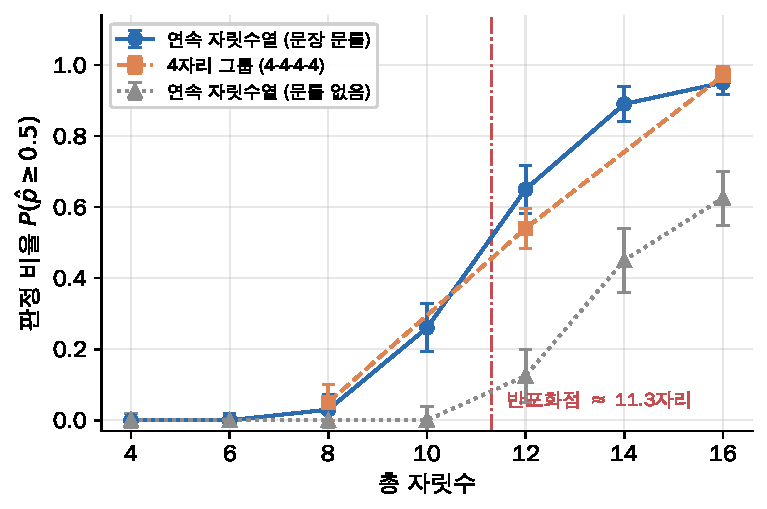
\includegraphics[width=\linewidth]{digit_curve.pdf}
\caption{통제 자극에 대한 자릿수 대 판정 비율 곡선 (v2 학습 세 시드의 평균 확률, 임계값 0.5,
오차 막대는 시드 간 표준편차). 총 자릿수를 맞추고 그룹 구조만 바꾼 곡선(주황)이 연속
자릿수열(파랑)과 겹치므로 그룹 경계는 결정에 관여하지 않는다. 문틀을 제거하면(회색) 곡선이
오른쪽으로 이동해, 숫자가 아닌 문틀 단어도 점수에 기여함을 보인다.}
\label{fig:digitcurve}
\end{figure}

\begin{table*}[!t]
\centering
\caption{헤드만 바꾼 변형의 비교 (v2, 시드 42/43/44 평균$\pm$표준편차, 임계값 0.5). 합성곱
몸통은 네 모델이 동일하다. 헤드는 차례로 균등 평균(전역 평균 풀링), 학습된 가중 평균(어텐션
풀링), 양방향 GRU 뒤 가중 평균, 같은 헤드에 시간 해상도를 네 배로 올린 것이다. ``순서''는 헤드가
시간축 순서를 볼 수 있는지, ``스텝''은 몸통 출력의 시간축 간격이다. ``일련번호 FPR''은 제품 일련번호(4-4-4, 12자리)를 학습에서 완전히 제외한 뒤 잰
미학습 오탐률이고, ``반포화점''은 통제 자극에서 연속 자릿수열 / 4자리 그룹 각각에 로지스틱을
적합한 값이다. 두 반포화점이 겹친다는 것은 그룹 구조가 결정에 관여하지 않는다는 뜻이다.}
\label{tab:seqhead}
\small
\setlength{\tabcolsep}{5pt}
\begin{tabular}{lccccccc}
\toprule
모델 & 순서 & 스텝 & F1 & Hard-neg FPR & ROC-AUC & 일련번호 FPR & 반포화점 연속/그룹 \\
\midrule
\texttt{simple\_cnn} & 없음 & 512\,ms & $0.859\pm0.011$ & $0.329\pm0.034$ & $0.938$ & $0.947\pm0.041$ & $11.3$ / $11.8$ \\
\texttt{attn\_cnn} & 없음 & 512\,ms & $0.915\pm0.003$ & $0.150\pm0.036$ & $0.971$ & $\mathbf{0.687\pm0.034}$ & $11.5$ / $11.7$ \\
\texttt{gru\_cnn} & \textbf{있음} & 512\,ms & $\mathbf{0.932\pm0.011}$ & $\mathbf{0.143\pm0.029}$ & $\mathbf{0.984}$ & $0.780\pm0.071$ & $11.2$ / $11.3$ \\
\texttt{gru\_cnn\_hires} & \textbf{있음} & \textbf{128\,ms} & $0.925\pm0.008$ & $0.166\pm0.031$ & $0.978$ & $0.813\pm0.034$ & $11.2$ / $11.4$ \\
\bottomrule
\end{tabular}
\end{table*}

\subsection{일반화: 화자와 PII 유형 (RQ3)}
\paragraph{화자 일반화.}
v1의 LOSO는 화자가 세 명뿐이라 폴드마다 두 명으로 학습하는 퇴화 조건이므로 v2와의 대비를 위한
참조점으로만 읽어야 한다. 그 조건에서도 미학습 화자에 대한 순위 성능은 아홉 폴드 전부에서
ROC-AUC $0.97$ 이상($0.992\pm0.008$)이었고 negative를 hard-negative로만 좁혀도 아홉 폴드 전부
$0.98$ 이상($0.996\pm0.004$)을 유지하여, 판별 신호 자체는 처음 보는 화자에게도 일관되게
일반화된다. 반면 고정 임계값 0.5에서 집계한 F1은 $0.616\pm0.280$으로 낮은데 이는 판별 실패가
아니라 임계값 오프셋 때문이다. 평균을 끌어내린 폴드는 재현율이 $0.068$--$0.175$로 낮은 대신
\emph{정밀도가 1.000}이었고 임계값을 0.2에서 0.8까지 옮겨도 hard-negative 오탐이 한 건도
발생하지 않았다. 문제는 오분류가 아니라 점수 분포 전체가 아래로 이동한 것이며, v1에서는 세
화자를 동시에 만족시키는 단일 임계값이 없다.

화자를 3명에서 14명으로 늘리자 고정 임계값 기준 F1이 $0.871\pm0.085$로 오르고 폴드 간
표준편차가 3분의 1로 줄었다(그림~\ref{fig:loso}). 14개 폴드의 F1 중앙값은 $0.893$으로 열한
폴드가 $0.87$ 이상이고, 재현율 중앙값은 $0.946$, ROC-AUC는 $0.969\pm0.021$로 열한 폴드가
$0.95$ 이상이다. 평균을 끌어내리는 것은 재현율이 $0.443$에 그친 폴드 하나이며, 이 폴드조차
정밀도 $0.934$, ROC-AUC $0.940$으로 순위 성능은 유지된다. 운용 관점에서 더 중요한 것은 폴드별로
검증셋에서 다시 고른 임계값이 $0.35$--$0.50$(평균 $0.444\pm0.043$)의 좁은 구간에 모두 모였고 그
임계값을 쓴 평균 F1 $0.862\pm0.083$이 고정 임계값 0.5의 $0.871\pm0.085$와 사실상 같다는
점이다. 화자가 바뀌어도 운용점을 다시 맞출 필요가 없다는 뜻이다. 다만 v1과 v2는 화자 수 외에
TTS 엔진과 PII 유형 수도 함께 달라졌으므로, 화자 수의 순효과를 분리하려면 동일 데이터에서 학습
화자 수만 바꾸는 실험이 필요하다.

\paragraph{PII 유형 일반화.}
각 PII 유형을 학습에서 완전히 제외하고 그 유형의 positive 225개 전부로 평가했을 때 세 유형 모두
재현율 $0.89$--$0.92$를 얻었다(표~\ref{tab:heldout}). 같은 유형을 학습에 포함했을 때의 재현율이
$0.85$--$1.00$인 점을 감안하면 유형을 통째로 빼도 재현율이 그 범위 아래로 크게 떨어지지 않는다.
학습 중 13자리 주민등록번호를 한 번도 보지 못한 모델이 그 유형의 $91.9\%$를 검출한다는 사실은
판별 근거가 유형별 자릿수 패턴의 암기가 아님을 보여준다. 다만 이 결과가 지지하는 일반화의
\emph{내용}은 \ref{sec:exp:decision}절의 결론과 함께 읽어야 한다. 제외된 유형들은 모두 자릿수
총량이 11--16으로 학습에 남은 유형들과 같은 구간에 있으므로, 이 실험이 보이는 것은 ``PII
형식''이라는 추상이 유형을 넘어 전이된다는 것이 아니라 자릿수 분량이라는 단일 축 위에서 학습된
결정 경계가 그 축의 같은 구간에 놓인 새 유형에도 적용된다는 것이다. 새 PII 유형 추가 시 재학습이
필요 없다는 운용상 함의는 유지되되, 그 유형의 자릿수 총량이 기존 구간 안에 있을 때에만
성립한다.

\begin{figure}[!t]
\centering
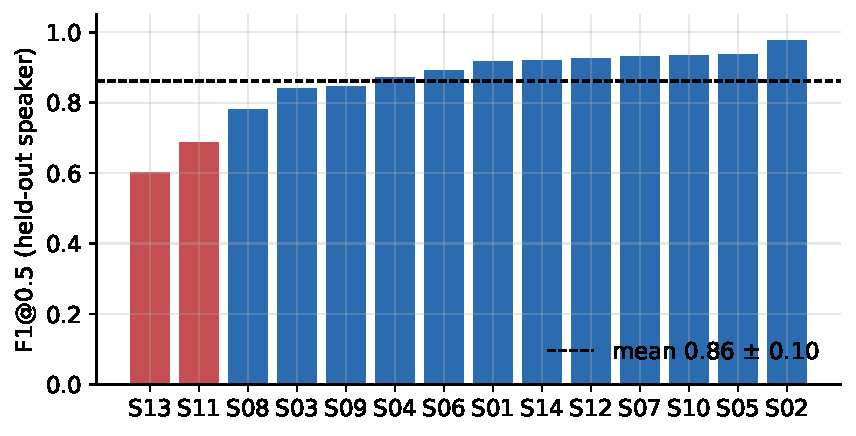
\includegraphics[width=\linewidth]{loso_folds.pdf}
\caption{v2 화자 분리(LOSO) 폴드별 F1(임계값 0.5, 14폴드 각각을 시드 42/43/44로 학습한 뒤 시드
평균, 오름차순 정렬). 붉은 파선은 14폴드 평균 $0.871$이다. 열한 폴드가 $0.87$ 이상이고 평균을
끌어내리는 것은 최좌측 한 폴드뿐이다. 화자가 세 명뿐인 v1의 같은 지표는 $0.616\pm0.280$으로,
화자 확장이 평균을 올리고 폴드 간 분산을 3분의 1로 줄였다(v1은 이 그림에 표시하지 않았다).}
\label{fig:loso}
\end{figure}

\begin{table}[!t]
\centering
\caption{held-out-PII 일반화 (v2, \texttt{simple\_cnn}, 시드 42/43/44 평균$\pm$표준편차,
임계값 0.5). 각 행은 해당 유형의 positive를 학습에서 완전히 제외한 뒤 그 유형의 positive
225개 전부에 대해 측정한 재현율이다. 오른쪽 열은 같은 유형이 학습에 포함되었을 때 v2-HN에서
측정한 재현율이며(주민 $n=52$, 카드 $n=81$, 계좌 $n=56$), 전화번호는 v2-HN에 positive가 남지
않아 비교 대상이 없다.}
\label{tab:heldout}
\footnotesize
\setlength{\tabcolsep}{4pt}
\begin{tabular}{lcccc}
\toprule
제외한 PII & 자릿수 & $n$ & held-out recall & (참고) 포함 시 \\
\midrule
주민번호 & 13 & 225 & $0.919\pm0.008$ & $0.846\pm0.042$ \\
카드     & 16 & 225 & $0.902\pm0.010$ & $1.000\pm0.000$ \\
계좌     & 12 & 225 & $0.893\pm0.038$ & $0.958\pm0.030$ \\
\bottomrule
\end{tabular}
\end{table}

\subsection{모델 규모: 경량 모델의 우위 (RQ5)}
네 모델은 검증 성능에서 구분되지 않는다. \texttt{simple\_cnn}, EfficientNet-B0, ConvNeXt-Tiny는
세 시드 대부분에서 검증 F1 $1.000$에 도달했고 MobileNetV3-Small도 $0.962$--$0.991$을 기록했다.
그럼에도 test F1은 $0.776$에서 $0.955$까지 벌어지므로 격차는 학습 데이터를 맞추는 능력이 아니라
처음 보는 템플릿으로의 일반화에서 발생한다. ConvNeXt는 두 번째 에폭에 이미 검증 F1 $1.000$에
도달하고 10에폭에서 조기 종료되었는데도 test F1은 $0.804\pm0.132$에 그쳤다. 임계값에 독립인
PR-AUC로 비교하면 \texttt{simple\_cnn}이 $0.998$, ConvNeXt가 $0.960\pm0.050$, MobileNetV3가
$0.954$이나 시드 3회의 표준편차가 $0.050$에 달하므로 이 차이는 통계적으로 유의하다고 주장할 수
없으며, 명확한 격차는 고정 임계값 F1과 지연에서 나타난다(표~\ref{tab:model}).

원인으로는 네 가지를 생각할 수 있으나 근거의 강도가 다르다. 실험으로 직접 관측된 것은 소량
데이터($\sim$2{,}000)에서 대형 모델의 학습이 불안정해진다는 점으로, ConvNeXt만 시드에 따라 F1이
$0.635$, $0.819$, $0.958$로 흔들려 표준편차 $\pm0.13$을 보인 반면 나머지 세 모델은 $\pm0.01$
수준이었다. ImageNet(자연 사진)과 멜 스펙트로그램의 도메인 불일치, 저수준 음향 패턴으로 풀리는
과제의 단순성, 작은 용량에 의한 암묵적 정규화는 해석적 가설이며 이를 가르려면 무작위 초기화
백본과의 대조 및 용량 스윕이 필요하다.

네 모델에 동일한 학습률 $10^{-4}$를 적용한 것이 사전학습 백본에 불리했을 가능성도 배제해야
한다. 전 계층 미세조정에 $10^{-4}$는 통상 과대하다고 알려져 있고 ConvNeXt의 큰 시드 간 분산이
바로 그 증상일 수 있기 때문이다. 이를 검정하기 위해 네 모델 각각에 $10^{-5}$, $3\times10^{-5}$,
$10^{-4}$를 시드 3회씩 적용하는 스윕을 수행하였다(총 36회, 결정성 고정). 결과는 두 가지를
말한다. 첫째, \emph{네 모델 모두 $10^{-4}$가 최적}이며 학습률을 낮추면 오히려 성능이 떨어진다.
사전학습 백본이라고 예외가 아니다. 둘째, ConvNeXt의 시드 간 불안정은 학습률을 낮춰도 해소되지
않는다. 표준편차는 $10^{-4}$에서 $\pm0.116$, $3\times10^{-5}$에서 $\pm0.072$, $10^{-5}$에서
$\pm0.067$로 줄지만 평균이 함께 떨어져 어느 설정에서도 \texttt{simple\_cnn}의 $0.952\pm0.012$에
미치지 못한다. 즉 ConvNeXt의 진동은 학습률 과대의 산물이 아니라 소량 데이터에서 대형 백본을
미세조정할 때의 성질로 보인다. 따라서 결론은 ``동일 예산·동일 설정에서''라는 단서를 ``각 모델에
가장 유리한 학습률을 고른 뒤에도''로 강화할 수 있다. 다만 비교군이 모두 ImageNet 사전학습
모델이므로, 이 실험이 지지하는 진술은 ``대규모 사전학습이 이 과제에 불리하다''가 아니라
``ImageNet 백본은 이 과제에서 60K 전용 CNN을 넘지 못한다''이며 오디오 도메인 사전학습
백본과의 비교는 남는다.

\begin{table*}[!t]
\centering
\caption{모델 효율성과 학습률 스윕 (v1 controlled 평가셋, 시드 42/43/44 평균$\pm$표준편차,
임계값 0.5, 결정성 고정). 파라미터는 학습 가능 파라미터 총수, 크기는 저장된 체크포인트 파일
용량, 지연은 NVIDIA A100 40GB에서 배치 크기 1로 $64\times157$ 입력을 워밍업 10회 뒤 50회
순전파한 평균(멜 스펙트로그램 추출 시간 제외)이다. 오른쪽 세 열의 각 셀은 해당 학습률로 3회
학습한 test F1이며, 굵게 표시한 값이 모델별 최적으로 네 모델 모두 $10^{-4}$이다.}
\label{tab:model}
\small
\setlength{\tabcolsep}{6pt}
\begin{tabular}{lcccccc}
\toprule
모델 & 파라미터 & 크기(MB) & GPU ms/window & F1 @ $10^{-5}$ & F1 @ $3\times10^{-5}$ & F1 @ $10^{-4}$ \\
\midrule
\textbf{simple\_cnn} & \textbf{60{,}706} & \textbf{0.26} & \textbf{0.34} & $0.628\pm0.048$ & $0.756\pm0.049$ & $\mathbf{0.952\pm0.012}$ \\
mobilenet\_v3\_small & 1{,}519{,}906 & 6.21 & 2.03 & $0.622\pm0.103$ & $0.776\pm0.003$ & $\mathbf{0.784\pm0.005}$ \\
efficientnet\_b0     & 4{,}010{,}110 & 16.34 & 2.92 & $0.832\pm0.016$ & $0.824\pm0.019$ & $\mathbf{0.877\pm0.045}$ \\
convnext\_tiny       & 27{,}821{,}666 & 111.35 & 2.32 & $0.776\pm0.067$ & $0.815\pm0.072$ & $\mathbf{0.852\pm0.116}$ \\
\bottomrule
\end{tabular}
\end{table*}

\begin{table*}[!t]
\centering
\caption{CNN 대 STT+NLP, 네 가지 Whisper 디코딩 설정 (v2 평가 분할, $n=336$, 임계값 0.5).
CNN은 시드 42/43/44 평균$\pm$표준편차이다. 이 분할의 hard-negative는 최대 8자리여서 형식 규칙을
건드리지 않으므로 STT+NLP의 ``형식만''과 ``형식+문맥''이 동일한 값을 낸다. 유형별 재현율에서
16자리 카드번호만 네 설정 모두에서 무너진다는 점이 핵심이다. 지연은 NVIDIA A100 40GB 기준으로
CNN이 배치 1의 윈도당 $0.344$\,ms(전처리 제외)이고, Whisper는 본 절의 재측정에서 빔 서치(5)
클립당 $0.541$\,s, 빔+프롬프트 $0.674$\,s였다.}
\label{tab:vs}
\small
\setlength{\tabcolsep}{6pt}
\begin{tabular}{lcccccc}
\toprule
접근 & F1 & Recall & Precision & 주민(13) & 계좌(12) & 카드(16) \\
\midrule
CNN (음향) & $0.859\pm0.011$ & $\mathbf{0.945\pm0.019}$ & $0.787\pm0.016$ & $0.846$ & $0.958$ & $\mathbf{1.000}$ \\
\midrule
STT+NLP, 기본        & $\mathbf{0.964}$ & $0.931$ & $\mathbf{1.000}$ & $1.000$ & $0.964$ & $0.864$ \\
STT+NLP, 프롬프트    & $0.956$ & $0.915$ & $\mathbf{1.000}$ & $1.000$ & $1.000$ & $0.802$ \\
STT+NLP, 빔 서치(5)  & $0.959$ & $0.921$ & $\mathbf{1.000}$ & $1.000$ & $0.946$ & $0.852$ \\
STT+NLP, 빔+프롬프트 & $0.959$ & $0.921$ & $\mathbf{1.000}$ & $1.000$ & $1.000$ & $0.815$ \\
\bottomrule
\end{tabular}
\end{table*}

\subsection{CNN 대 STT+NLP (RQ4)}
동일 인스턴스(v2 평가 분할, $n=336$)에서 두 접근을 비교하면 강점이 뚜렷하게 갈린다
(표~\ref{tab:vs}). STT+NLP는 정밀도 $1.000$과 F1 $0.964$로 앞서고, CNN은 재현율($0.945$ 대
$0.931$)과 세 자릿수 빠른 지연으로 앞선다. 이 분할의 hard-negative는 최대 8자리여서 형식 규칙을
아예 건드리지 않으므로 STT+NLP의 오탐률이 $0.000$이고 문맥 결합이 개입할 여지도 없다. 형식이
충돌하는 10자리 주문번호가 평가에 포함된 제거 이전 분할에서는 ``형식만''의 오탐률이 $0.218$,
문맥 결합 시 $0.063$으로 문맥이 형식 충돌을 해결하는 효과가 나타난다. 즉 STT+NLP의 정밀도 우위
역시 평가 분할의 자릿수 구성에 의존한다.

논문이 STT의 약점을 ``구조적''이라고 부르려면 최소한 서로 다른 디코딩 설정에서 같은 실패가
재현되어야 한다. 16자리 카드번호 재현율은 기본·프롬프트·빔 서치·결합의 네 설정에서 각각
$0.864$, $0.802$, $0.852$, $0.815$로 프롬프트나 빔 서치가 이 실패를 개선하지 못하며, 오히려
형식 예시를 준 프롬프트 설정이 가장 낮다. 반면 13자리 주민등록번호는 네 설정 모두 $1.000$이다.
즉 실패는 디코딩 탐색의 문제가 아니라 자릿수가 길어질수록 전사가 숫자를 병합·분절·누락하는 데서
오는 것이며 ``구조적''이라는 규정이 유지된다. 같은 인스턴스에서 CNN의 카드 재현율은 세 시드 모두
$1.000$이다. 유형별로 나누면 상보성이 선명해진다. CNN이 우위를 보이는 지점은 정확히 전사가
취약한 긴 숫자열(카드 16자리: $1.000$ 대 $0.802$--$0.864$)이고, STT+NLP가 앞서는 지점은 짧고
문맥 키워드가 뚜렷한 유형(주민 13자리: $1.000$ 대 $0.846\pm0.042$)이다. 이 상보성을 어떤 논리 연산으로 쓸지는 \ref{sec:discuss:combine}절에서 클립 단위 판정을 실제로
결합해 가른다.

이 비교에서 STT+NLP 쪽 조건도 밝혀 둔다. 합성음에서는 Whisper 전사가 거의 완벽하여(일반 발화
449개 기준 WER 중앙값 $0$, 평균 $0.079$, 완전일치 $80.8\%$) STT+NLP 성능은 best-case 상한이다.
완전일치하지 않은 클립이 $19.2\%$라는 점은 남으며, 중앙값이 0이라는 사실은 전사 오류가
사라졌다는 뜻이 아니라 소수 구간에 집중되어 있다는 뜻이다. 그 소수 구간이 하필 긴 숫자열이라는
점이 카드번호 재현율 $0.802$--$0.864$로 나타난다.

\subsection{프리필터 운용점}
프리필터의 목적은 목표 재현율을 지키면서 STT 호출을 줄이는 것이다. v1 평가셋에서는 고정 임계값
0.5에서 이미 재현율 $0.927$, 정밀도 $0.986$을 유지하며 STT 호출을 51.5\% 줄일 수 있고, 임계값을
0.3으로 낮추면 재현율 $0.994$에서 44.9\%, 0.2에서는 재현율 $0.998$에서 41.6\%를 절감한다. 반대로
임계값을 0.7로 올리면 세 시드 모두 정밀도 $1.000$과 hard-negative 오탐 0건을 유지한 채 평균
62\%를 절감하지만 재현율이 $0.728$로 떨어져 PII의 27\%를 놓친다. 프리필터로서 실제로 쓸 수 있는
구간은 재현율을 지키는 저임계값 쪽이며 그 구간에서 41--45\%의 절감이 확보된다.

숫자를 포함한 발화만으로 구성된 v2-HN에서도 임계값 $0.375\pm0.059$에서 재현율 $0.981\pm0.005$를
유지하며 STT 호출을 $24.2\%$ 줄일 수 있다(표~\ref{tab:prefilter}). 주목할 점은 이 임계값들이
모두 검증 분할의 확률 분위수만으로 정해졌고 test를 참조하지 않았음에도 목표를 초과 달성했다는
것이다. \ref{sec:data:split}절에서 밝혔듯 val과 test의 hard-negative 카테고리는 서로 겹치지
않으므로, 이는 운용점이 학습·검증에서 한 번도 보지 못한 종류의 비PII 숫자열에도 이식됨을
보여준다. 다만 임계값 자체의 시드 간 변동은 작지 않으므로($0.99$ 목표에서 $0.214\pm0.047$)
프리필터 임계값은 배포 시점의 검증 데이터에서 다시 정하는 것이 안전하다. v2-HN의 호출률은 모든
입력이 숫자를 포함하는 최악 트래픽을 가정한 값이라 운용 절감률을 크게 과소평가하며, 실제
트래픽에서의 값은 \ref{sec:discuss:cost}절의 비용 모형으로 일반화한다.

\begin{table}[!t]
\centering
\caption{프리필터 운용점 (v2-HN, \texttt{simple\_cnn}, 시드 42/43/44 평균$\pm$표준편차). 각 열의
임계값은 검증 분할에서 목표 재현율에 해당하는 분위수로 정한 값이다. STT 호출률은 클립 점수가
임계값 이상이어서 후단 STT로 넘어가는 클립의 비율이며 $1-\text{호출률}$이 절감률이다. v2-HN에는
숫자 없는 easy-negative가 없으므로 여기의 호출률은 최악 트래픽 가정값이다.}
\label{tab:prefilter}
\footnotesize
\setlength{\tabcolsep}{3.5pt}
\begin{tabular}{lccc}
\toprule
목표 재현율 & 0.99 & 0.95 & 0.90 \\
\midrule
임계값        & $0.214\pm0.047$ & $0.375\pm0.059$ & $0.500\pm0.028$ \\
Recall        & $0.996\pm0.005$ & $0.981\pm0.005$ & $0.942\pm0.020$ \\
Precision     & $0.665\pm0.014$ & $0.728\pm0.015$ & $0.799\pm0.006$ \\
Hard-neg FPR  & $0.646\pm0.044$ & $0.472\pm0.037$ & $0.304\pm0.014$ \\
STT 호출률    & $0.843\pm0.022$ & $0.758\pm0.019$ & $0.663\pm0.015$ \\
\bottomrule
\end{tabular}
\end{table}

\begin{table*}[!t]
\centering
\caption{협대역·코덱·잡음 열화 후 성능 (v2 평가 분할 $n=336$, 임계값 0.5, 시드 42/43/44
평균$\pm$표준편차). 열화는 평가 시점에만 가하며 ``기본''은 깨끗한 음성만으로 학습한 모델,
``증강''은 학습 데이터의 절반에 대역 제한·$\mu$-law·통과대역 잡음을 섞어 학습한 모델이다.
STT+NLP는 기본 디코딩 설정의 ``형식+문맥'' 변형이며 단일 실행이다. 통과대역 잡음은
300--3400\,Hz로 제한하고 SNR을 대역 내 전력비로 정의한 것으로 전화망이 실제로 전달하는
조건이며, 맨 아래 두 행의 전대역 잡음은 신호가 없는 4--8\,kHz에 잡음의 절반이 떨어지므로 표적
도메인에서는 발생하지 않는다.}
\label{tab:degrade}
\small
\setlength{\tabcolsep}{6pt}
\begin{tabular}{lcc|cc|c}
\toprule
 & \multicolumn{2}{c|}{CNN 기본} & \multicolumn{2}{c|}{CNN 잡음 증강} & STT+NLP \\
조건 & F1 & Recall & F1 & Recall & F1 \\
\midrule
clean (16\,kHz) & $0.859\pm0.011$ & $0.945\pm0.019$ & $0.807\pm0.010$ & $0.885\pm0.026$ & $0.964$ \\
8\,kHz 왕복 & $0.849\pm0.016$ & $0.910\pm0.030$ & $0.819\pm0.015$ & $0.834\pm0.025$ & $0.947$ \\
G.711 ($\mu$-law) & $0.831\pm0.013$ & $0.910\pm0.031$ & $0.806\pm0.015$ & $0.840\pm0.002$ & $0.956$ \\
\midrule
\;+ 통과대역 잡음 20\,dB & $0.754\pm0.020$ & $0.931\pm0.069$ & $0.757\pm0.002$ & $0.843\pm0.002$ & $0.962$ \\
\;+ 통과대역 잡음 10\,dB & $0.622\pm0.169$ & $0.746\pm0.352$ & $\mathbf{0.770\pm0.010}$ & $0.838\pm0.044$ & $0.950$ \\
\;+ 통과대역 잡음 5\,dB & $0.491\pm0.348$ & $0.667\pm0.471$ & $\mathbf{0.777\pm0.024}$ & $0.785\pm0.096$ & $0.932$ \\
\midrule
\;+ (참고) 전대역 잡음 20\,dB & $0.542\pm0.116$ & $0.418\pm0.127$ & $0.435\pm0.231$ & $0.381\pm0.303$ & $0.967$ \\
\;+ (참고) 전대역 잡음 10\,dB & $0.615\pm0.111$ & $0.589\pm0.180$ & $0.620\pm0.100$ & $0.653\pm0.227$ & $0.953$ \\
\bottomrule
\end{tabular}
\end{table*}

\subsection{협대역·코덱·잡음 열화}\label{sec:exp:degrade}
지금까지의 실험은 깨끗한 16\,kHz 녹음에서 이루어졌지만, 실제로 쓰일 곳은 전화망이다. 전화는
소리를 훨씬 좁은 주파수 대역으로 눌러 보내고 압축까지 하므로 조건이 다르다.\footnote{전화망은
대략 300--3400\,Hz 구간만 전달하며 이를 협대역(narrowband)이라 한다. G.711은 그 신호를 8\,kHz로
표본화해 8비트로 압축하는 표준 코덱이다. 통과대역(passband)은 채널이 실제로 통과시키는 주파수
구간을 뜻하며, SNR(신호 대 잡음비)은 신호 전력이 잡음 전력의 몇 배인지를 데시벨로 나타낸 값으로
클수록 깨끗하다.} 새 데이터
수집 없이 이 격차의 크기를 재기 위해 v2 평가 분할의 클립을 전화망 조건으로 열화시킨 뒤 동일
체크포인트로 재평가하였다(표~\ref{tab:degrade}). 결과는 두 요인의 기여를 뚜렷하게 분리한다.
\emph{대역 제한과 코덱은 거의 무해하다.} 8\,kHz 리샘플 왕복만으로는 F1이 $0.859\to0.849$,
ROC-AUC가 $0.938\to0.920$으로 거의 변하지 않고 G.711 $\mu$-law 양자화를 더해도 $0.831$ /
$0.914$에 머문다. 자릿수 낭독의 판별 정보가 4\,kHz 이하의 저역 포먼트와 음절 리듬에 실려 있음을
생각하면 자연스러운 결과이다.

\paragraph{잡음을 어느 대역에 넣는가가 결론을 바꾼다.}
가산 잡음 조건에서는 잡음의 대역이 결정적이다. 협대역 채널을 통과한 신호는 4\,kHz 이상 에너지가
사실상 0이므로(본 데이터의 G.711 클립 336개에서 4\,kHz 이상 에너지 비율의 중앙값
$1.3\times10^{-5}$, 최댓값 $1.3\times10^{-4}$) 전대역 백색잡음을 공칭 SNR로 주입하면 잡음 전력의
절반이 \emph{신호가 전혀 없는 대역}에 떨어진다. 그 대역은 64채널 멜 필터뱅크의 절반을 차지하므로
모델 입력에는 크게 반영되지만 실제 전화망은 이런 잡음을 전달하지 못한다. 따라서 잡음은 전화
통과대역(300--3400\,Hz)으로 제한하고 SNR도 대역 내 전력비로 정의하는 것이 옳으며, 본 절은 두
방식을 모두 보고한다.

이 구분이 결론을 뒤집는다. 전대역 잡음에서는 공칭 SNR 20\,dB만으로 재현율이 $0.945\to0.418$로
무너지지만 통과대역 잡음 20\,dB에서는 $0.931\pm0.069$로 거의 유지된다. 두 SNR은 정의가 달라 직접
비교할 수 없는데, 통과대역 SNR은 대역 내 전력비이고 G.711 클립에서 300--3400\,Hz가 총전력의 약
$52\%$이므로 통과대역 20\,dB는 전체 전력 기준 약 $24$\,dB에 해당한다. 이 $4$\,dB 차이만으로는
$0.418$과 $0.931$의 간극이 설명되지 않으므로 지배적 요인은 잡음의 대역 배치이다. 전대역
조건에서 SNR을 10\,dB로 더 낮추면 재현율이 오히려 $0.589$로 오르는 비단조성 역시, 손실이 정보량이
아니라 점수 분포 이동에서 온다는 해석과 맞는다. 즉 ``가산 잡음이 음향 프리필터를 무너뜨린다''는
서술은 표적 도메인이 물리적으로 만들 수 없는 대역 외 잡음에 기댄 것이었다. 통과대역 조건에서
실제로 무너지는 것은 재현율이 아니라 \emph{정밀도와 운용점의 안정성}이다. hard-negative
오탐률이 $0.329\to0.689$로 오르고, SNR을 10\,dB와 5\,dB로 낮추면 시드 간 재현율이 각각
$[0.989, 1.000, 0.249]$, $[1.000, 1.000, 0.000]$로 극단적으로 갈린다. 판별 능력도 ROC-AUC
$0.938\to0.804/0.770/0.742$로 유의하게 떨어지지만(우연 대비 여유가 $0.438\to0.242$로 $45\%$
감소) 시드 간 재현율이 $1.000$과 $0.000$으로 갈리는 폭은 그 감소만으로 설명되지 않는다. 지배적
요인은 점수 분포가 잡음 수준에 따라 예측 불가능하게 이동하여 고정 임계값이 무의미해지는 데
있다. 프리필터 관점에서 재현율 손실과 정밀도 손실은 비용이 전혀 다르다. 전자는 PII 누락이고
후자는 STT 호출 증가일 뿐이므로, 통과대역 조건의 열화는 앞의 서술이 시사하던 것보다 훨씬 덜
치명적이다.

\paragraph{잡음 증강 학습으로 회복되는가.}
위 열화는 모두 평가 시점에만 가해졌고 모델은 깨끗한 16\,kHz 합성음만 보았다. 관측된 저하가 과제의
한계인지 학습 조건 불일치인지 가르기 위해 학습 데이터의 절반에 확률적으로 대역 제한, $\mu$-law
양자화, 통과대역 잡음(SNR 5--25\,dB)을 섞어 동일 절차로 재학습하였다(시드 3회). 다만 이 실험이
무엇을 보이는지는 정확히 한정해야 한다. 증강에 쓴 통과대역 잡음은 평가에 쓴 것과 대역
상수·필터·잡음원·SNR 정의가 같고 학습 SNR 범위 $[5, 25]$\,dB가 평가점 $\{20, 10, 5\}$을 모두
포함하므로, 아래 회복치는 \emph{정합 조건에서의 상한}이며 처음 보는 잡음 종류로의 일반화를
뜻하지 않는다. 실제로 학습에 넣지 않은 전대역 잡음에서는 증강이 오히려 성능을 낮춘다(F1
$0.542\to0.435$).

그 한정 아래에서 효과는 분명하다. 통과대역 잡음 조건에서 F1은 SNR 20, 10, 5\,dB에 대해 각각
$0.757$, $0.770$, $0.777$로 \emph{SNR에 거의 무관하게} 평평해지고 재현율도 $0.843$, $0.838$,
$0.785$로 안정된다. 기본 모델의 $0.754$, $0.622$, $0.491$과 비교하면 SNR 5\,dB에서 F1이 $0.29$
오르고 시드 간 표준편차도 $\pm0.348$에서 $\pm0.024$로 줄어 운용점 불안정이 해소된다. 대가는
깨끗한 조건의 성능으로, F1이 $0.859\to0.807$, 재현율이 $0.945\to0.885$, ROC-AUC가
$0.938\to0.883$으로 내려간다. 또 SNR 20\,dB에서는 증강의 이득이 사실상 없다(F1
$0.754\to0.757$, 재현율은 $0.931\to0.843$으로 오히려 내려간다). 즉 증강은 \emph{낮은 SNR에서의
붕괴와 시드 간 불안정}을 없애는 대신 깨끗한 구간의 성능을 내주는 거래이며, 잡음 하 붕괴가 최소한
정합 조건에서는 과제의 본질이 아니라 학습 조건 불일치였음을 보인다.

동일 클립에 STT+NLP 경로를 적용하면 이 경로가 전 조건에서 훨씬 견고하다. 통과대역 잡음
20/10/5\,dB에서 F1이 $0.962$/$0.950$/$0.932$로 5\,dB에서만 소폭 내려가고 16자리 카드 재현율도
$0.840$/$0.790$/$0.728$로 유지된다. 대규모 실음성으로 학습된 ASR과 깨끗한 합성음 1{,}800개로
학습된 60{,}706 파라미터 CNN을 견주는 비대칭 비교이므로 이 격차를 두 \emph{접근}의 차이로 읽어서는
안 되지만, 운용 판단에는 그대로 반영되어야 한다. 따라서 프리필터의 운용 전제는 ``잡음이 없어야
한다''가 아니라 ``잡음 조건으로 증강 학습하고, 깨끗한 구간의 F1 $0.05$를 대가로 지불한다''이며,
그럼에도 잡음 구간에서 프리필터가 STT+NLP보다 더 많이 잃는다는 사실 자체는 남는다. 또한 여기서
쓴 잡음은 정상 백색잡음이므로 실제 통화의 배경 대화·음악 같은 비정상 잡음에서 같은 결과가
나온다고 단정할 수 없다.

\section{논의}\label{sec:discuss}

\subsection{정밀도 약점의 원인 진단}
\ref{sec:exp:decision}절의 결론을 정밀도 문제로 옮기면 진단이 단순해진다. 모델이 재는 것이
자릿수 낭독의 분량이라면, PII와 그 분량이 겹치는 비PII 숫자열은 이 결정 축 위에서 구분할 수
없다. 실제로 제품 일련번호(12자리)는 계좌번호(12자리)와 총량이 정확히 같고 미학습 오탐률이
$0.947$이다. 다만 두 유형은 그룹 구조가 4-4-4 대 3-3-6으로 다르므로, 이 상한을 넘어설 여지가 원리적으로
닫혀 있지는 않다. 그러나 그 여지가 표현 구조를 바꾸는 것만으로 열리지는 않는다는 점이
\ref{sec:exp:decision}절의 순서 헤드 실험에서 확인되었다. 순서를 인지하는 헤드는 정밀도를 크게
올리지만(hard-negative 오탐률 $0.329\to0.143$) 그룹 경계는 여전히 쓰지 않으며, 얻은 것은 자릿수
축 위의 더 정확한 근사이다. 따라서 정밀도 개선의 남은 레버는 표현이 아니라 (a) 문맥 단서 결합,
(b) 그룹 구조만이 유일한 판별 단서가 되도록 설계한 학습 데이터 쪽에 있다. 문맥을 보는 후단이 필요한 이유는 그와 별개로,
형식이 같아도 문맥상 PII가 아닌 경우가 존재하기 때문이다.

이 관점은 단일 분할에서 측정한 hard-negative 오탐률을 어떻게 읽어야 하는지도 결정한다. 그 값은
모델의 속성이라기보다 \emph{평가 분할에 어떤 카테고리가 남았는지}의 함수이다. 같은 학습 절차로
같은 데이터를 쓰되 분할만 달리한 두 계열을 비교하면 655초 오염 클립을 제거한 분할에서는
$0.329\pm0.034$, 제거 이전 분할에서는 $0.566\pm0.041$로 $0.24$가 벌어진다. 전자의 평가
카테고리는 \{생일 $0.167$, 수 세기 $0.404$, 송장번호 $0.462$\}이고 후자는 \{좌석번호 $0.222$,
수 세기 $0.577$, 주문번호 $0.896$\}이다. 템플릿 그룹 단위 부트스트랩\footnote{가진 표본에서 복원추출로 가짜 표본을 여러 번 만들어
지표가 얼마나 흔들리는지 보는 방법이다. 여기서는 클립이 아니라 템플릿 그룹을 통째로 다시
뽑는다. 클립 단위로 뽑으면 같은 템플릿에서 나온 클립들이 서로 독립이 아니어서 불확실성을
실제보다 작게 보고하게 되기 때문이다.}으로 재면 이 불확실성이 정량화된다. 오탐률의 95\% 구간은 $[0.167, 0.466]$, 정밀도는 $[0.363, 0.967]$, F1은
$[0.519, 0.960]$으로 시드 간 표준편차($\pm0.034$, $\pm0.016$, $\pm0.011$)보다 한 자릿수 크다.
다만 이 평가 분할의 템플릿 그룹은 여섯 개(positive 세 유형, hard-negative 세 카테고리)뿐이므로
재표집 단위가 적고, 따라서 이 구간은 정확한 피복률을 갖는 신뢰구간이라기보다 \emph{불확실성의
하한}으로 읽어야 한다. 그럼에도 시드 분산과의 자릿수 차이는 이 정도 표본으로도 분명하다. 즉
v2의 지배적 불확실성 축은 학습 난수가 아니라 평가에 어떤 템플릿이 들어오는가이며, 단일 분할의
오탐률 하나를 모델의 정밀도로 인용해서는 안 된다. 표~\ref{tab:heldcat}의 카테고리별 미학습
오탐률이 이 지표를 대체해야 한다.

v1에서 같은 지표가 $0.006$이었던 것도 같은 틀로 설명된다. v1의 positive는 전화번호(11자리)
하나뿐이고 v1 hard-negative의 자릿수 총량은 대부분 5 이하여서 자릿수 총량 축에서 두 클래스가
거의 겹치지 않는다. v2에서 계좌(12)와 카드(16)를 추가하자 12자리 제품 일련번호와 10자리
주문번호가 곧바로 충돌 구간으로 들어왔다. 두 수치의 비를 악화 배수로 읽는 것은 과대해석이며,
``PII 유형을 늘리면 자릿수 총량이 겹치는 negative가 늘어난다''가 정확한 진술이다.

보정의 성격도 함께 확인된다. 보정 파라미터는 검증 분할에서 적합하고 test에서 평가하였다. 기대
보정 오차(Expected Calibration Error, ECE)는 $0.098\pm0.012$로 절대적으로 낮지 않지만 온도
스케일링($T=0.67\pm0.07$)을 적용해도 $0.097\pm0.014$로 변화가 없고 Platt
스케일링~\cite{guo2017calibration}은 $0.110\pm0.010$으로 오히려 악화된다. 온도 스케일링은 순위를
보존하는 단조 변환이므로 임계값 0.5에서의 재현율·정밀도·호출률도 보정 전후로 동일하다. 운용상
사후 보정 단계를 추가할 실익이 없다는 뜻이고, 진단상으로는 정밀도 개선의 레버가 보정이 아니라
(a) 문맥 단서 결합, (b) 자릿수 총량이 겹치는 충돌형 hard-negative의 강화 학습에 있음을 뜻한다.

\subsection{결합 설계: 캐스케이드 대 합집합}\label{sec:discuss:combine}
두 경로를 어떻게 이어 붙일 것인가. 흔히 쓰는 방식은 음향 모델을 앞에 두어 후보를 거르고
살아남은 것만 전사하는 직렬 구조(캐스케이드)이다. 그런데 \ref{sec:exp:decision}절의 결론은 그
전제를 흔든다. 음향 모델은 ``PII 후보 선별기''가
아니라 ``긴 자릿수 낭독 검출기''이며, 콜센터 트래픽에서 주문번호나 송장번호는 PII보다 오히려 더
자주 등장한다. 그럼에도 표~\ref{tab:vs}의 유형별 재현율은 두 경로의 실패가 \emph{반대 방향}임을
보인다. 전사는 자릿수가 길수록 무너지고(카드 16자리 $0.864$) 음향 경로는 길수록 잘한다($1.000$).
이 상보성을 어떤 논리 연산으로 쓸지가 설계 선택이다.

클립 단위 판정을 실제로 결합하여 네 설계를 같은 인스턴스에서 비교하였다(표~\ref{tab:combine}).
캐스케이드는 음향 경로가 통과시킨 클립만 전사하므로 최종 판정이 두 경로의 논리곱이 되고, 합집합은
둘 중 하나라도 켜지면 positive로 둔다.

결과는 \emph{캐스케이드의 재현율 손실이 임계값의 함수}임을 보인다. 관례적 기본값 $\tau=0.5$에서는
캐스케이드가 STT 단독보다 나쁘다. 놓친 PII가 $13.0$건에서 $23.3$건으로 늘고, 임계값을 올릴수록
악화된다($\tau=0.9$에서 $41.0$건). 프리필터가 PII의 일부를 후단이 보기도 전에 버리기 때문이다.
그러나 임계값을 낮추면 이 손실은 사라진다. $\tau=0.1$에서 캐스케이드의 재현율은 $0.931$로 STT
단독과 \emph{정확히 같고}, 그러면서도 STT 호출을 줄인다(\ref{sec:discuss:cost}절에서 정량화한다).
요컨대 캐스케이드는 검출 성능을 더해 주지 못하지만, 임계값만 제대로 고르면 검출 성능을 깎지도
않는다. 캐스케이드의 가치는 순수하게 비용에 있으며, 기본값 $0.5$를 그대로 쓰는 것이 문제였다.

반대로 \emph{합집합은 놓친 PII를 거의 없앤다}. 같은 조건에서 $13.0$건이 $0.0$건이 되고, 정밀도가
높은 순서 헤드 모델을 $\tau=0.9$로 쓰면 재현율 $0.993$, 정밀도 $0.979$로 STT 단독($0.931$ /
$1.000$)을 재현율에서 크게 앞서면서 정밀도는 $0.021$만 내준다. 규제 준수 관점에서 놓친 PII는
규제 사건이고 오탐은 불필요하게 가려진 구간이므로, 이 거래는 대개 유리한 쪽이다.

합집합의 이점은 열화 조건에서 더 뚜렷하다. 통과대역 잡음 SNR 5\,dB에서 음향 경로 단독은 재현율이
$0.667\pm0.471$로 시드에 따라 붕괴하지만, 합집합은 $0.958\pm0.060$으로 유지된다. 전사 경로가
받쳐 주므로 음향 경로의 불안정이 최종 판정으로 전파되지 않는다. 같은 조건에서 캐스케이드는 반대로
음향 경로의 실패를 증폭하여 놓친 PII가 $79.0$건에 이른다.

요컨대 음향 경로의 운용 역할은 셋으로 갈리며, 이 데이터가 지지하는 강도가 서로 다르다.
(i) \emph{PII 분류기}는 성립하지 않는다. 결정 축이 자릿수 분량이라 형식을 읽지 못한다.
(ii) \emph{비용 프리필터}는 조건부로 성립한다. 숫자 없는 발화에 대한 오탐률이 $F_e=0.085$이므로
그런 발화가 많은 트래픽에서는 잘 걸러 내지만, 숫자 밀집 구간에서는 가치가 붕괴하고 재현율까지
잃는다. (iii) \emph{재현율 안전망}이 가장 강하게 지지된다. 5초 윈도당 $0.344$\,ms로 전사 경로가
놓치는 긴 숫자열을 회수하며, 이것이 두 경로의 상보성을 실제로 쓰는 유일한 결합이다.

\begin{table}[!t]
\centering
\caption{음향 경로와 STT+NLP 경로의 결합 (v2-HN $n=336$, positive 189, Whisper 기본 디코딩의
``형식+문맥'' 변형, 음향 경로는 시드 42/43/44 평균$\pm$표준편차). 캐스케이드는 두 판정의 논리곱,
합집합은 논리합이다. ``놓친 PII''는 positive 189건 가운데 검출되지 않은 수이다.}
\label{tab:combine}
\footnotesize
\setlength{\tabcolsep}{4pt}
\begin{tabular}{lccc}
\toprule
설계 & Recall & Precision & 놓친 PII \\
\midrule
\multicolumn{4}{l}{\emph{깨끗한 조건, \texttt{simple\_cnn} ($\tau=0.5$)}} \\
STT+NLP 단독 & $0.931$ & $\mathbf{1.000}$ & $13.0$ \\
음향 단독 & $0.945\pm0.019$ & $0.787\pm0.016$ & $10.3$ \\
캐스케이드 & $0.877\pm0.019$ & $\mathbf{1.000}$ & $23.3$ \\
\textbf{합집합} & $\mathbf{1.000\pm0.000}$ & $0.797\pm0.017$ & $\mathbf{0.0}$ \\
\midrule
\multicolumn{4}{l}{\emph{깨끗한 조건, \texttt{gru\_cnn} ($\tau=0.9$)}} \\
캐스케이드 & $0.783\pm0.019$ & $\mathbf{1.000}$ & $41.0$ \\
\textbf{합집합} & $\mathbf{0.993\pm0.002}$ & $0.979\pm0.008$ & $\mathbf{1.3}$ \\
\midrule
\multicolumn{4}{l}{\emph{통과대역 잡음 SNR 5\,dB, \texttt{simple\_cnn} ($\tau=0.5$)}} \\
STT+NLP 단독 & $0.873$ & $\mathbf{1.000}$ & $24.0$ \\
음향 단독 & $0.667\pm0.471$ & $0.389\pm0.275$ & $63.0$ \\
캐스케이드 & $0.582\pm0.412$ & $0.667\pm0.471$ & $79.0$ \\
\textbf{합집합} & $\mathbf{0.958\pm0.060}$ & $0.722\pm0.197$ & $\mathbf{8.0}$ \\
\bottomrule
\end{tabular}
\end{table}

\subsection{비용 모형과 손익분기}\label{sec:discuss:cost}
프리필터로 쓸 때의 가치는 절감된 STT 호출 비용과 놓친 PII의 기대 손실을 함께 놓아야 판단할 수
있다. 아래에서 ``손익분기''란, PII 한 건을 놓쳤을 때의 손실이 STT 한 번 호출하는 값의 몇 배까지
커져도 프리필터를 쓰는 편이 남는가를 뜻한다. 이 배수가 클수록 안전한 설계이다. 발화 하나를 단위로, PII 포함
비율을 $p$, 비PII 발화 가운데 비PII 숫자열을 포함하는 비율을 $q$, 프리필터 재현율을 $R$, 비PII
숫자열과 숫자 없는 발화에 대한 오탐률을 각각 $F_h$, $F_e$, STT 단가를 $c_s$, 프리필터 단가를
$c_f$, PII 1건을 놓쳤을 때의 기대 손실을 $c_m$이라 하면 STT 호출률과 발화당 순절감은
\begin{align}
\rho &= pR + (1-p)\bigl(qF_h + (1-q)F_e\bigr), \\
\text{순절감} &= (1-\rho)c_s - c_f - (1-R)\,p\,c_m
\end{align}
이고, 프리필터가 이득이 되는 조건은
\begin{equation}
\frac{c_m}{c_s} < \frac{(1-\rho) - c_f/c_s}{(1-R)\,p}
\end{equation}
이다.

측정값을 대입한다. \ref{sec:exp}장에서 $\tau=0.5$일 때 $R=0.945$, $F_h=0.329$를 얻었다. 숫자 없는
발화에 대한 오탐률 $F_e$는 v2 평가 분할에 easy-negative가 없어 그 분할에서는 잴 수 없으나, LOSO
폴드를 모으면 각 시드마다 easy-negative 449개 전부가 \emph{학습에 쓰이지 않은 화자}의 클립으로
한 번씩 채점되므로 화자 수준에서 누수 없는 추정이 된다. 이 값은 $\tau=0.5$에서 $F_e=0.085$로,
v1 controlled test에서 얻어 쓰던 $0.020$보다 네 배 크다. 아래 계산은 보수적인 $0.085$를 쓴다.
다만 LOSO는 화자만 분리하고 easy-negative의 문장 템플릿 12종은 학습에도 등장하므로, 이 값 역시
처음 보는 비숫자 발화에 대해서는 낙관적일 수 있다. 단가비는 지연
실측(윈도당 $0.344$\,ms 대 클립당 수백 ms)에서 $10^{-3}$ 수준이나 보수적으로
$c_f/c_s=5\times10^{-3}$으로 둔다. 표~\ref{tab:cost}가 $p$와 $q$를 바꾼 결과이고, 표~\ref{tab:tau}는 트래픽을 콜센터형으로 고정한 채
\emph{임계값}을 바꾼 결과이다. 후자가 운용상 더 중요한 표이다. 관례적 기본값 $\tau=0.5$는 재현율
$0.945$에 절감 $80\%$를 주지만 발화 1{,}000건마다 PII $2.7$건을 놓친다. 임계값을 $0.2$로
낮추면 재현율이 $0.996$으로 오르면서도 절감이 $56\%$ 남고, $0.1$에서는 \emph{재현율 $1.000$에
절감 $40\%$}가 된다. 즉 이 데이터에서 프리필터는 ``재현율을 지키려면 절감을 포기해야 하는''
장치가 아니며, 놓치는 PII 없이 STT 호출을 $40\%$ 줄이는 구간이 실재한다. 반대로 기본값 $0.5$를
그대로 쓰면 손익분기가 $292$배로 내려가는데, PII 1건 누락이 규제 사건인 환경에서 이 배수는 사실상
충족되지 않는다. 콜센터 트래픽에서 PII를 담은 발화가 5\%, 비PII 발화의 30\%가 어떤 숫자든
포함한다고 보면 $\tau=0.5$에서 STT 호출률은 $0.198$로 떨어져 비용의 $80\%$가 절감되고, PII 1건을 놓치는 손실이 STT 단가의 약
$292$배를 넘지 않는 한 이득이다.
반대로 v2-HN처럼 모든 발화가 숫자를 포함하는 극단($q=1$, $p=0.5$)에서는 절감이 36\%로 줄고
손익분기 배수도 13으로 낮아진다. 즉 \ref{sec:exp}장이 보고한 ``숫자 포함 트래픽에서 24\%
절감''은 이 접근의 하한이며 실제 운용 트래픽에서는 절감률이 훨씬 크다. 동시에 이 표는 프리필터가
유리하지 않은 영역도 명시한다. PII 밀도가 매우 높거나($p\!\to\!0.5$) 한 건의 누락 비용이 STT
단가의 수십 배를 넘는 규제 환경에서는 재현율을 더 올리거나(표~\ref{tab:prefilter}의 $0.99$
운용점) 프리필터를 쓰지 않는 편이 낫다.

열화 조건에서의 값도 같은 $F_e$로 계산하였다. 잡음 증강 학습 모델을 전화 통과대역 SNR 20\,dB에
놓으면 표~\ref{tab:degrade}의 $R=0.843$과 그 조건의 hard-negative 오탐률 $F_h=0.494$가 되어,
$p=0.05$, $q=0.3$에서 호출률이 $0.198\to0.239$, 손익분기가 $292\to96$으로 내려간다. 다만 이
계산은 $F_e$를 깨끗한 조건 값 $0.085$ 그대로 썼다. 잡음에서 $F_h$가 오르면 $F_e$도 오르는 것이
자연스러우므로 $96$은 낙관적 추정이며, $F_e$를 세 배($0.255$)로 두면 $82$까지 내려간다. 그럼에도 깨끗한 조건의 손익분기를 그대로 운용 근거로 삼아서는 안 된다는 결론과, 여유가
여전히 두 자릿수라는 사실은 유지된다. 요컨대 2단계 구조는 무조건 우월한 설계가 아니라 입력
품질에 조건부인 설계이며, 잡음이 심한 구간에서는 프리필터를 우회하고 전량 전사하는 운용 분기를
함께 두는 편이 안전하다.

\begin{table}[!t]
\centering
\caption{임계값에 따른 재현율과 절감 (콜센터형 트래픽 $p=0.05$, $q=0.30$, \texttt{simple\_cnn},
시드 42/43/44 평균). $R$과 $F_h$는 v2-HN에서, $F_e$는 LOSO 폴드를 모은 easy-negative
449개$\times$3시드에서 측정하였다. ``놓친 PII''는 발화 1{,}000건당 기대값이고, 손익분기는 이득이
유지되는 $c_m/c_s$의 상한이다. $\tau=0.1$에서는 세 시드 모두 positive를 하나도 놓치지 않아
손익분기가 정의되지 않는다.}
\label{tab:tau}
\footnotesize
\setlength{\tabcolsep}{4pt}
\begin{tabular}{ccccccc}
\toprule
$\tau$ & $R$ & $F_h$ & $F_e$ & 절감률 & 놓친 PII & 손익분기 \\
\midrule
$0.10$ & $\mathbf{1.000}$ & $0.805$ & $0.484$ & $39.9\%$ & $\mathbf{0.0}$ & --- \\
$0.20$ & $0.996$ & $0.662$ & $0.298$ & $56.3\%$ & $0.2$ & $3{,}167$ \\
$0.30$ & $0.988$ & $0.558$ & $0.189$ & $66.6\%$ & $0.6$ & $1{,}070$ \\
$0.50$ & $0.945$ & $0.329$ & $0.085$ & $\mathbf{80.2\%}$ & $2.7$ & $292$ \\
$0.70$ & $0.841$ & $0.134$ & $0.038$ & $89.5\%$ & $7.9$ & $112$ \\
$0.90$ & $0.587$ & $0.018$ & $0.001$ & $96.4\%$ & $20.6$ & $46$ \\
\bottomrule
\end{tabular}
\end{table}

\begin{table}[!t]
\centering
\caption{프리필터 비용 모형 ($\tau=0.5$: $R=0.945$, $F_h=0.329$, $F_e=0.085$, $c_f/c_s=0.005$). 순절감은
STT 단가 $c_s$를 1로 둔 발화당 값이고, 손익분기는 이득이 유지되는 $c_m/c_s$의 상한이다. $p$는
PII 포함 발화 비율, $q$는 비PII 발화 중 숫자 포함 비율이다.}
\label{tab:cost}
\footnotesize
\setlength{\tabcolsep}{5pt}
\begin{tabular}{ccccc}
\toprule
$p$ & $q$ & STT 호출률 $\rho$ & 발화당 순절감 & 손익분기 $c_m/c_s$ \\
\midrule
0.01 & 0.3 & $0.166$ & $0.829$ & $1{,}516$ \\
0.05 & 0.1 & $0.151$ & $0.844$ & $309$ \\
0.05 & 0.3 & $0.198$ & $0.797$ & $292$ \\
0.20 & 0.3 & $0.316$ & $0.679$ & $62$ \\
0.20 & 1.0 & $0.452$ & $0.543$ & $50$ \\
0.50 & 1.0 & $0.637$ & $0.358$ & $13$ \\
\bottomrule
\end{tabular}
\end{table}

\subsection{프라이버시 관점}
CNN 프리필터는 민감 텍스트를 생성하지 않고 이진 신호만 산출하므로 프리필터에서 걸러지는 비PII
발화는 전사되지 않는다. 다만 이 이득의 범위는 정확히 좁혀 읽어야 한다. 걸러지는 것은 정의상
PII를 담지 않은 발화이고, 실제 PII를 담은 발화는 재현율이 높을수록 오히려 빠짐없이 후단으로
넘어가 그대로 전사된다. 따라서 이 구조가 줄이는 것은 \emph{PII 평문이 생성되는 건수}가 아니라
\emph{전사 텍스트가 생성되는 전체 건수}이며, 프라이버시 논거로는 PII 노출 축소가 아니라 데이터
최소화에 해당한다. \ref{sec:intro}장에서 지적한 ``전사 텍스트가 유출 표면이 된다''는 문제 가운데
본 접근이 해소하는 부분은 비PII 발화가 만드는 표면에 한정되며, PII 발화가 만드는 표면은
프라이버시 보존 전사~\cite{ahmed2020preech} 같은 별도 수단으로 다루어야 한다. 두 접근이
배타적이지 않다는 점은 오히려 결합의 근거가 된다.

\section{한계 및 향후 연구}\label{sec:limit}
본 결과는 합성 TTS 데이터에 한정된다. \ref{sec:exp:degrade}절의 열화 실험은 이 한계 가운데 채널
요인(대역, 코덱, 가산 잡음)의 크기를 구체적인 수치로 바꾸어 놓았지만, 원리적으로 제거할 수 없는
층위가 하나 남는다. 본 연구의 통제 장치 전부, 즉 자릿수 강제 변환, hard-negative 투입, 캐리어
결합, 화자 풀 통일은 모두 \emph{합성 분포 안에서} 작동하므로 합성 분포 자체가 지름길인 층위는
데이터셋 내부 통제로 건드릴 수 없다. 이 점이 특히 중요한 이유는 \ref{sec:exp:decision}절이 특정한
결정 변수가 ``등간격으로 연쇄되는 음절의 개수''이기 때문이다. TTS는 숫자열을 사람보다 훨씬
규칙적인 운율과 일정한 그룹 휴지로 읽으며, 이는 하필 모델이 쓰는 바로 그 신호를 실제보다
뚜렷하게 만드는 방향이다. 실제 상담 통화에서는 ``공일공$\ldots$ 어 잠시만요$\ldots$
일팔이사''처럼 자릿수 낭독이 비유창성으로 끊기는 것이 기본이므로 실음성에서의 성능은 채널
열화만으로 설명되는 것보다 더 떨어질 수 있다. 소수의 화자에게 자릿수열을 읽히는 소규모 실녹음
세트만 확보해도 이 층위를 처음으로 검증할 수 있으며, 이를 최우선 후속 과제로 둔다. STT+NLP 쪽
성능 또한 합성음 best-case 기준이므로 같은 재평가가 필요하나, \ref{sec:exp:degrade}절의 결과는
두 경로가 대칭적으로 나빠지지 않으리라는 점을 이미 시사한다. 따라서 실통화 검증의 초점은 ``둘 다
얼마나 나빠지는가''가 아니라 ``프리필터가 어느 SNR 구간까지 STT 대비 이득을 남기는가''에
맞추어야 한다.

데이터 설계 측면에서는 세 가지 제약이 있다. 첫째, 14화자는 설계된 합성 화자로 최근접 쌍의
분리도가 제한적이어서 실제 화자 다양성과는 다르다. 둘째, 문장 템플릿의 절대 수가 적으며 이 축이
본 연구의 \emph{지배적 불확실성}이다. v2의 positive는 16개, v1은 14개 템플릿에서 파생되었고
hard-negative는 10개 카테고리 생성기로 만들어졌다. 분할을 템플릿 단위로 나누어 학습과 평가 사이의
템플릿 암기는 차단했지만, 일반화가 검증된 범위는 이 템플릿 집합이 포괄하는 문형에 한정된다.
셋째, 모든 발화가 단일 화자의 완결된 한 문장이며 화자 교대와 중첩 발화, 되묻기와 자기수정 같은
비유창성, 숫자열이 여러 발화 구간에 걸쳐 끊어져 발화되는 상황은 포함되지 않았다.

방법 측면에서도 세 가지를 남긴다. 첫째, 클립 점수를 윈도 최댓값으로 집계하는 방식은 클립이
길수록 윈도 수가 늘어 오탐 확률이 단조 증가한다. 본 데이터의 클립은 중앙값 4.6초로 대부분 윈도
한두 개에 담기므로 이 편향이 드러나지 않았으나, 수 분 길이의 실통화에 적용하려면 상위 $k$개
평균이나 윈도 수로 보정한 집계, 또는 발화 단위 분절 후 적용을 검토해야 한다. 둘째, 저진폭 노이즈
패딩은 길이 단서를 완전히 제거하지 못한다. 5초보다 짧은 클립은 윈도 안에서 음성이 차지하는
비율로 길이를 노출하며 hard-negative 내부에서 길이와 점수의 상관이 $0.482$로 남는다. 클래스 간 길이는 맞추어져 있어 주 결론에는 영향이 없으나, 길이 통제를 완전하게 하려면 윈도보다
짧은 클립을 만들지 않도록 데이터를 설계하는 편이 낫다. 아울러 윈도 길이 5초는 가장 긴 대상인
16자리 카드번호 낭독을 한 윈도에 담을 수 있는 값으로 정한 것이며, 윈도 길이와 이동 간격에 대한
민감도 분석은 수행하지 않았다. 셋째, 비교 대상인 STT+NLP의 ``형식+문맥'' 변형은 비PII
키워드 목록을 본 데이터셋의 hard-negative 카테고리에 맞추어 구성하였다. 이는 규칙 기반 경로에
유리한 조건이므로 그 정밀도 역시 상한으로 읽어야 하며, 처음 보는 유형의 비PII 숫자열이 등장하면
``형식만'' 변형 쪽에 가까워질 것으로 예상된다.

\ref{sec:exp:decision}절의 순서 헤드 실험은 두 가지를 후속 과제로 남긴다. 첫째, 그룹 경계가
학습되지 않는 원인이 표현 구조가 아님은 확인했으나 어느 층위인지는 좁히지 못했다. 학습 분할의
제품 일련번호가 50개뿐이라는 데이터 규모와, TTS가 그룹 휴지를 사람보다 규칙적으로 넣어 휴지가
``자릿수 낭독 중''이라는 신호로만 쓰이고 경계 위치는 무시되었을 가능성이 남는다. 이를 가르려면
자릿수 총량을 고정하고 그룹 구조만 판별 단서가 되도록 설계한 학습셋이 필요하다. 둘째, 본 논문의
나머지 실험(LOSO, held-out-PII, 열화, 비용 모형)은 모두 \texttt{simple\_cnn}으로 수행되었으므로,
hard-negative 오탐률이 절반 이하인 순서 헤드로 주 모델을 교체한 재실행이 필요하다.

향후 과제로 (i) 소규모 실녹음을 이용한 합성 분포 층위의 검증, (ii) 비정상 잡음으로의 증강 확대와
잡음 조건 임계값 재보정, (iii) 그룹 구조만이 판별 단서가 되는 학습셋 설계와 문맥 결합 모델, (iv)
화자·TTS·템플릿 다양성 확대와 템플릿 단위 분할 설계 보완, (v) 긴 오디오를 위한 집계 방식 재설계,
(vi) 오디오 도메인 사전학습 백본(PANNs, AST)과의 비교를 제시한다.

\section{결론}\label{sec:conclusion}
STT 없이 멜 스펙트로그램과 경량 CNN만으로 PII 형식 숫자열을 높은 재현율로 선별할 수 있음을 통제
실험으로 확인하였다. 성능이 지름길 단서에서 온 것이 아님은 길이 정렬, hard-negative 투입, 캐리어
문장의 조건부 검정이라는 세 통제로 확인하였다.

그 위에서 본 연구가 도달한 가장 구체적인 결론은 모델의 결정 함수를 특정한 것이다. 카테고리별
미학습 오탐률과 통제 자극 실험은 판별 근거가 자릿수 그룹 구조가 아니라 등간격 단음절 연쇄의
분량임을 보인다. 이는 겸손한 서술이 아니라 더 강한 주장이다. ``형식을 학습했다''는 진술은 같은
분량을 갖는 비PII 숫자열 하나로 반박되지만, ``결정 경계가 그 분량 축 위 어디에 있는가''는
측정값이므로 같은 방식으로 반박되지 않는다. 그리고 이 결론은 한 구조의 우연이 아니다. 헤드를 어텐션 풀링과 양방향 GRU로 바꾸고 시간
해상도를 네 배로 올려도, 나아가 자릿수 총량이 같고 그룹 구조만 다른 쌍(제품 일련번호 4-4-4 대
계좌 3-3-6)이 학습 분할에 직접 감독으로 들어 있는데도, 어느 구조도 그룹 경계를 결정에 쓰지
않았다. 대신 같은 축 위의 근사가 정밀해져 F1이 $0.859$에서 $0.932$로 올랐다. 즉 본 논문이 보고한
수치는 접근법의 상한이 아니라 헤드의 상한이며, 결정 축 자체는 이 설정에서 바뀌지 않는다.

일반화는 화자와 PII 유형 두 축 모두에서 성립하였으며, 특히 학습에서 완전히 제외한 PII 유형도
재현율 $0.89$--$0.92$로 검출되었다. 표준 경로와의 비교는 두 접근이 실패하는 지점이 서로 어긋남을
드러내고, 16자리 카드번호에 대한 전사 취약성이 네 가지 디코딩 설정에서 모두 재현됨을 확인하였다.
다만 이 상보성을 쓰는 방식은 결합 연산에 달려 있다. 클립 단위 판정을 결합해 보면 음향 경로를
앞단 필터로 두는 캐스케이드는 관례적 임계값 $0.5$에서 재현율이 STT 단독보다 낮고(놓친 PII
$23.3$건 대 $13.0$건), $\tau=0.1$까지 낮추어야 손실이 사라진다. 그 지점에서도 STT 호출은 가정한 콜센터형 트래픽에서
$39.9\%$, 모든 발화가 숫자를 포함하는 평가셋 자체에서는 $8.5\%$ 줄어든다. 반면 두 판정의 합집합은 놓친 PII를 $0.0$건으로 없앤다. 따라서 음향 경로는
검출 성능을 더해 주는 후보 선별기가 아니라 \emph{비용을 줄이는 필터이자 재현율을 지키는
안전망}이며, 어느 쪽으로 쓰든 임계값을 목적에 맞게 다시 골라야 한다. 남은 과제는 실음성 검증과 잡음 강건화이며, 열화 실험은 이 가운데 채널 요인의 크기를
수치로 제시하고 잡음을 전화 통과대역으로 제한해야 표적 도메인의 조건이 된다는 점과 잡음 증강
학습이 SNR 5\,dB까지 성능을 평평하게 만든다는 점을 함께 보였다.

\bibliographystyle{unsrt}
\bibliography{refs}

\end{document}
